%%%%%%%%%%%%%%%%%%%%%%%%%%%%%%%%%%%%%%%%%%%%%%%%%%%%%%%%%%%%%%%%%%%%%%%%%%%%%%%
%%% Modèle de thèse électronique pour les sciences (c) Jean Hare 2017
%%%%%%%%%%%%%%%%%%%%%%%%%%%%%%%%%%%%%%%%%%%%%%%%%%%%%%%%%%%%%%%%%%%%%%%%%%%%%%%
%%% Format personnalisé avec %& :  doit figurer  seul sur la 1ière ligne %
%%&"mythesis"
%%% Les trois commentaires spéciaux ci-dessous sont destinés à l'éditeur TeXWorks
% !TeX encoding = UTF-8
% !TeX program = pdflatex
% !TeX spellcheck = en_GB
\documentclass[a4paper,11pt]{book} %ADD diffusion OR archiv for final versions
\usepackage[utf8]{inputenc}
%\usepackage[latin9]{inputenc}
\usepackage{xspace}			  
\usepackage[french]{babel}
\usepackage[T1]{fontenc}
\usepackage{lmodern}
\usepackage[margin=28mm,includeheadfoot,bindingoffset=5mm]{geometry}
\usepackage{algorithm}
%\usepackage[]{algorithm2e}
\usepackage{algorithmic}
\usepackage{upgreek}
\input{./preamb/preamb-graph.tex}
\input{./preamb/preamb-math.tex}
\input{./preamb/preamb-util.tex}
\input{./preamb/preamb-titles.tex}
%%%%%%%%%%%%%%%%%%%%%%%%%%%%%%%%% HYPERREF %%%%%%%%%%%%%%%%%%%%%%%%%%%%%%%%%%%%
\usepackage[pagebackref]{hyperref}
\hypersetup{colorlinks,linkcolor=DarkBlue,anchorcolor=DarkRed,%
pdfdisplaydoctitle=true,pdfpagemode=UseOutlines,%
bookmarksnumbered=true,bookmarksopen=true}
%%%%%%%%%%%%%%%%%%%%%%%%%%%%%%%% TOOLS DURING WRITONG (to be removed) %%%%%%%%%%
%% !TeX encoding = UTF-8
%%% préamble pour les paquet à usabe temporaires %%%
%%% Généaration de fake text, et marquage des versions de travail  : à supprimer ! %%%
\usepackage{lipsum} 
\usepackage{blindtext}
\blindmathtrue
\AddToShipoutPictureBG{% Add picture to background of every page
  \AtPageLowerLeft{%
    \raisebox{3\baselineskip}{\makebox[\paperwidth][c]{Version \today, \currenttime}}%
}}
\usepackage[notref,notcite]{showkeys}
\usepackage[pdftex]{changebar}
\usepackage{versions}          % permet d'activer ou non certains environnements

\AfterEndPreamble{\nocite{*}}


%%%%%%%%%%%%%%%%%%%%%%%%%%%% END OF CUSTOM FORMAT%%%%%%%%%%%%%%%%%%%%%%%%%%%%%%
%\csname{} endofdump \endcsname
%%%%%%%%%%%%%%%%%%%%%%%%%%%% SELECTED INCLUDES  %%%%%%%%%%%%%%%%%%%%%%%%%%%%%%%%
%\includeonly{chap3}
%%%%%%%%%%%%%%%%%%%%%%%%%%%%%% CUSTOM PACKAGES %%%%%%%%%%%%%%%%%%%%%%%%%%%%%%%%
\usepackage{thcover}% or \usepackage{thcoverpsl} for psl thesis
\usepackage{versionswitch}
%%%%%%%%%%%%%%%%%%%%%%%%%%%%%%%%%%%%%%%%%%%%%%%%%%%%%%%%%%%%%%%%%%%%%%%%%%%%%%%
\begin{document}
%%%%%%%%%%%%%%%%%%%%%%%%%%%%%% PAGES LIMINAIRES %%%%%%%%%%%%%%%%%%%%%%%%%%%%%%%
%\frontcover % requires thcover.sty loaded and thcoverdata.tex filled
\frontmatter
%\tableofcontents
% !TeX encoding = UTF-8
% !TeX spellcheck = fr_FR
% !TeX root = mythesis.tex
\chapter{Introduction}

Some intro text

%%%%%%%%%%%%%%%%%%%%%%%%%%%%%%%%%%% TEXT BODY %%%%%%%%%%%%%%%%%%%%%%%%%%%%%%%%%
\mainmatter

%% !TeX encoding = UTF-8
% !TeX spellcheck = fr_FR
% !TeX root = mythesis.tex
\chapter{Quasi-particle signature in FQHE}

Le projet de charge fractionnaires détectée par bruit RF

\section{\texorpdfstring{Le set-up de mesure de bruit}{}}

\section{\texorpdfstring{Les calculs d'Ines-Safi}{}}

\section{\texorpdfstring{Les résultats de conductances et de bruit BF}{}}

\section{\texorpdfstring{Les résultats de bruit RF}{}}

%% !TeX encoding = UTF-8
% !TeX spellcheck = fr_FR
% !TeX root = mythesis.tex
\chapter{Electron wavefunctions tomography}

It is about the project of tomo

\section{\texorpdfstring{Un cas 1e th froid pas de périodicité}{}}

\section{\texorpdfstring{Un cas 1e pour de vrai}{}}

\section{\texorpdfstring{exploration en largeur}{}}

\section{\texorpdfstring{exploration deux électrons}{}}

\section{\texorpdfstring{exploration en electrons puis trous}{}}

\section{\texorpdfstring{exploration autre forme exponentielle}{}}


%% !TeX encoding = UTF-8
% !TeX spellcheck = en_GB
% !TeX root = mythesis.tex
\chapter{Edge-magneto-plasmon squeezing}

Le projet de squeezing

\begin{figure}[hptb]
	\begin{center}
		\begin{tabular}{c}
			 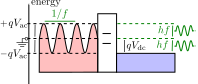
\includegraphics[width = 6.5 cm]{./chap3/noise_schematics}
		\end{tabular}
	\end{center}
	
	\caption{\textbf{title.}}
	\label{fig: squeezing principle schematics}
\end{figure}

\section{Experimental set-up}

In this section the electrical circuits used to perform the measurements are presented.
The measurements have been realized in two steps, the first measurement is the noise generated by the RF sinus voltage excitation, and the second measurement is the noise generated by the DC voltage excitation.
These two electrical circuits are drawn in figure Fig. \ref{fig: set-up chap 3}.

\begin{figure}
	\centering
	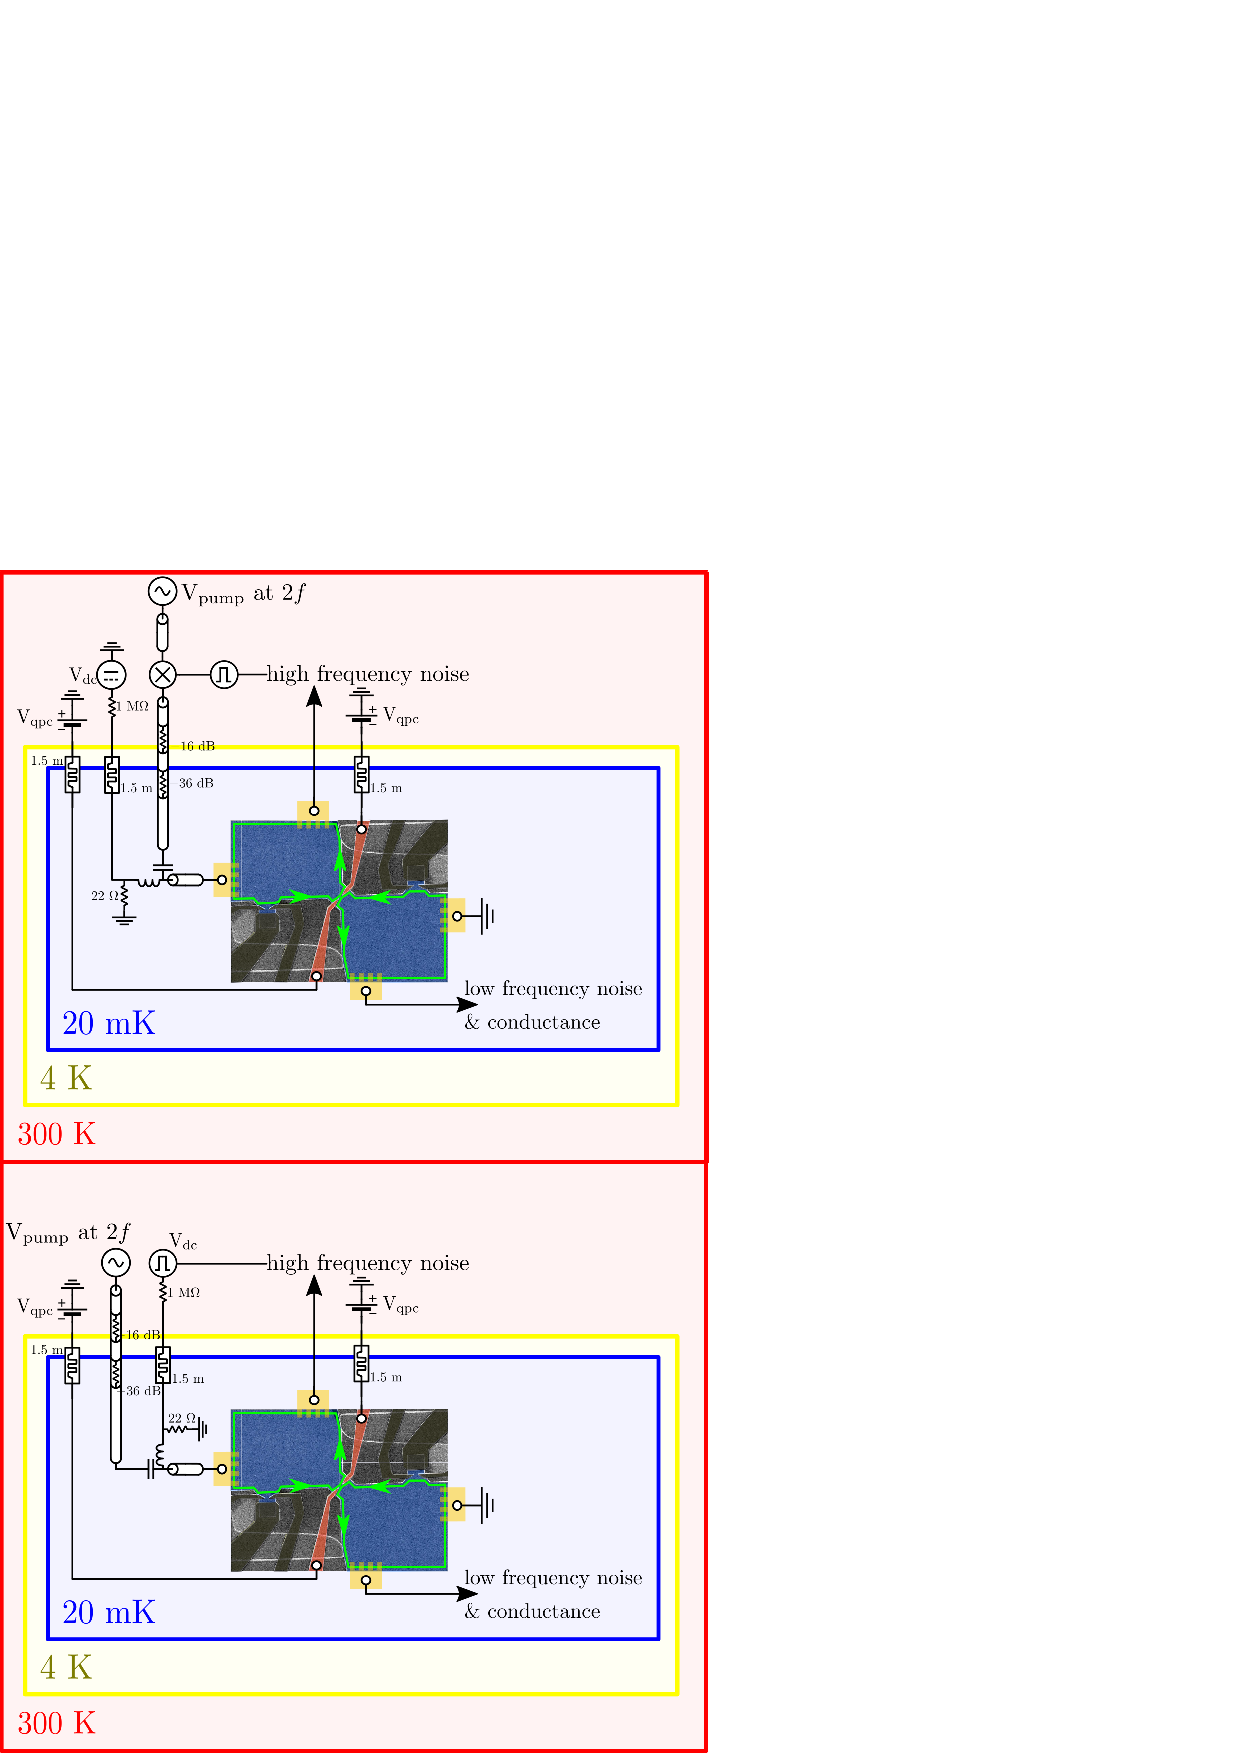
\includegraphics[width = 10cm]{./chap3/set-up_bruit_RF_pour_squeezing.pdf}
	\caption{\textbf{Electrical circuits for edge-magneto-plasmon squeezing measurement.} The circuit in the top panel is used to measure the high frequency noise of the pump sinus voltage $V_{\mathrm{pump}}$ at twice the measurement frequency $2f$. The pump voltage is modulated with a mixer by a square voltage at $\sim 230$ Hz included between $0$ V and $0.75$ V. The modulation signal is used in the RF noise measurement set-up represented in figure Fig. \ref{fig: le set-up chap2}. The pump voltage is added to a DC voltage with a bias tee at cold temperature. The circuit in the bottom panel enables to measure the high frequency noise of a DC voltage with the pump voltage. The square voltage at $\sim 230$ Hz is used for both the modulation and demodulation and to apply the DC voltage as it is included between $0$ V and $V_{\mathrm{dc}}$.}
	\label{fig: set-up chap 3}
\end{figure}

\subsection{Measurement of noise generated by the RF sinus voltage}

The top part of the figure Fig. \ref{fig: set-up chap 3} represents the circuit to measure the effect on the noise of the RF signal.
The measurement lines are not represented since they have been explained in the precedent chapters.
The low frequency noise is measured thanks to the circuit drawn in chapter 2, and the high frequency noise is measured thanks to the circuit drawn in chapter 1.
The high frequency measurement circuit uses a modulation of the source, which is done by a low frequency square voltage and a mixer.
The mixer is used as a switch for the RF sinus source as it is controlled by the low frequency square signal alternating between $0$ V and $0.75$ V.
After passing through the mixer, the RF sinus voltage, noted $V_{\mathrm{pump}}$, is attenuated and added to a DC voltage before exciting an edge-channel.
The DC voltage source is independent of the low frequency source generating the modulation signal, so the voltage $V_{\mathrm{DC}}$ is continuously applied on the edge-channel.
This set-up allows to measure the noise difference between two situations when both RF sinus voltage source and DC voltage source are turned on and when only DC voltage source is turned on.
This set-up access the excess high frequency noise of the voltage pump over the thermal noise when $V_{dc}$ is set at 0 V.

\subsection{Measurement of noise generated by the DC voltage}

The bottom part of the figure Fig. \ref{fig: set-up chap 3} is a drawing of the set-up used to probe how the variation of the voltage $V_{dc}$ affects the high frequency noise.
For this purpose the modulated signal is the DC Voltage $V_{dc}$, which is a square signal between 0 V and $V_{dc}$ produced by a low frequency function generator.
It is attenuated by a voltage divider and added to the RF sinus before its connection with an edge-channel.
In this set-up the RF sinus voltage is continuously generated, the high frequency noise measured is the difference of noise between both RF sinus and DC voltage are applied and only the noise of the RF sinus.
This connexion allows to measure the reduction of the high frequency noise compared to the noise of the RF sinus alone.

The two sources DC and RF are modulated separately because non-linearities of elements in the high frequency noise measurement chain.
These non-linearities generate strong parasitic signals in case of simultaneous modulation which blind the measurement.
The separated modulation cancel these parasitic and still allows to recover the total high frequency noise reduction compared to thermal noise by adding the two measurements.
Only the thermal noise is not measured but it is very close to vacuum noise because $\dfrac{hf}{k_{B}T} ...$, the thermal energy is too low to generate high frequency noise.

\section{Squeezed state evidence in quantum hall regime by high frequency noise measurement}

\subsection{Spectroscopy characterization of RF sinus excitation}

\begin{figure}[hptb]
	\begin{center}
		\begin{tabular}{c c c c}
			(a) & & (b) & \\
			& 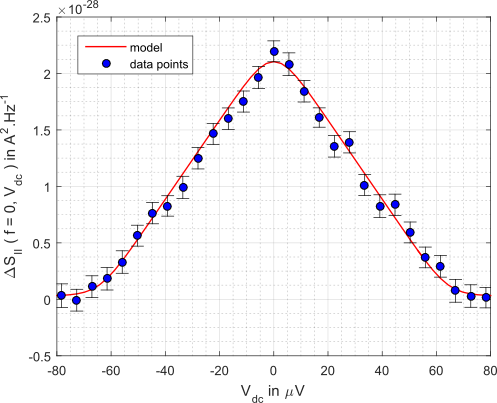
\includegraphics[width = 6.5 cm]{./chap3/LF_noise_pump_vs_V_dc} &
			& 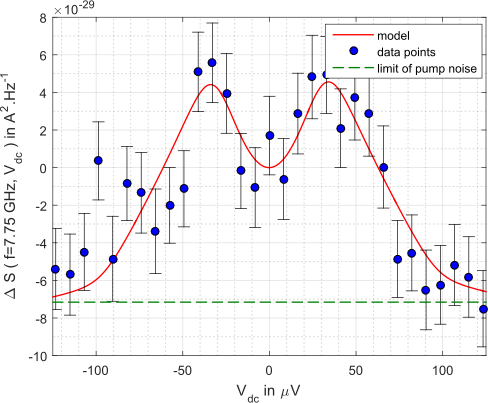
\includegraphics[width = 6.5 cm]{./chap3/RF_noise_pump_vs_V_dc}
		\end{tabular}
	\end{center}
	
	\caption{\textbf{Pump contribution to excess noise as a function of bias voltage.} \textbf{(a)} Low frequency noise difference between shot noise with the pump voltage and shot noise without pump $\Delta S_{II} = S_{II}\left(V_{\mathrm{ac}}\right) - S_{II}\left(V_{\mathrm{ac}}=0\right)$. \textbf{(b)} High frequency noise difference between noise with pump voltage and without pump voltage. For this measurement the high frequency measurement set-up of figure Fig. \ref{fig: le set-up chap2} is changed. The local oscillator, I-Q mixers, low pass filters, diodes, differential amplifiers, are replaced by a band pass filter around $f = 7.75$ GHz and a diode. With this change the magnitude of the total noise is measured instead of its real and imaginary part. The bias is still modulated so the value at $V_{dc} = 0$ is still substracted. The measured noise is then $\Delta\left|S_{II}\right|\left(V_{\mathrm{ac}}\right)-\Delta\left|S_{II}\right|\left(V_{\mathrm{ac} = 0}\right)$. And it tends the opposite of noise of the pump at large bias represented by the green dashed line. The models for both panels are computed thanks to the Wigner distribution of the pump.}
	\label{fig: noise pump vs Vdc}
\end{figure}

In the chapter ... the Wigner function of RF excitations is determined with low frequency noise measurements.
The control of the RF sinus voltage used in this chapter relies in part on the same measurements.
Only the first measurement of low frequency noise when both the RF source signal and the DC voltage bias are applied on the quantum point contact is performed.
The consistency between the model and the measurements gives the parameters of the RF sinus voltage.
In the panel (a) of figure \ref{fig: noise pump vs Vdc} the measurement is performed with a RF sinus voltage of frequency $f = 15.5$ GHz and an amplitude $V_{ac}$ around 38 $\upmu$V at the quantum point contact level.
The agreement between the model line and the data points confirms the values of amplitude and frequency of the RF sinus.

With this set-up we can performed the same kind of measurement by recording the high frequency noise instead of the low frequency one.
In this measurement we are interested in the magnitude of the noise, so the elements from the I-Q mixers to the differential amplifiers are replaced by a band pass filter around $f = 7.75$ GHz and a diode. 
The data points of obtained are plotted in the panel (b) of figure \ref{fig: noise pump vs Vdc}.
The noise without the RF voltage is subtracted to the noise from both RF and DC voltage to get the excess noise in the same way as the low frequency measurements.
The noise value at $V_{\mathrm{dc}} = 0$ V differs from the low frequency noise because the DC voltage is modulated in the high frequency set-up.
This modulation leads to a zero value of the measured excess noise at $V_{\mathrm{dc}} = 0$ V because it is automatically subtracted by the modulation.
The data points are consistent with numerical calculation in red line whose high $V_{\mathrm{dc}}$ limit is minus the high frequency noise of the RF sinus alone.
That limit is displayed on the graph by a green dashed line and will be directly measured in the next paragraph.
This second measurement adds an other indication of the amplitude and frequency of the RF sinus, and gives a first hint of the noise value added by the RF sinus. 

\subsection{High frequency noise of a RF sinus}

\begin{figure}[hptb]
	\begin{center}
		\begin{tabular}{c c c c}
			(a) & & (b) & \\
			& 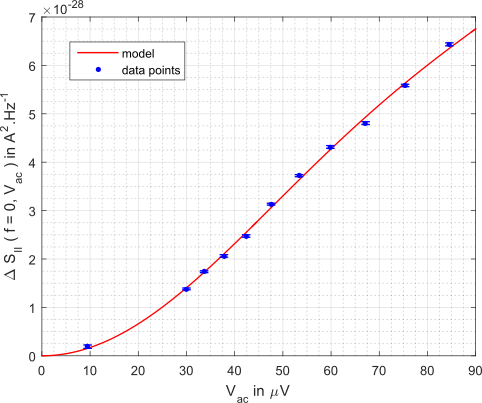
\includegraphics[width = 6.5 cm]{./chap3/LF_noise_vs_pump_amp} &
			& 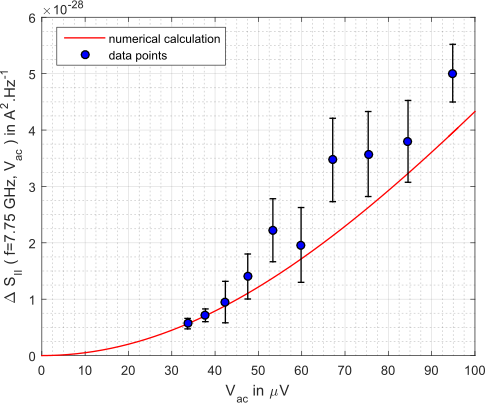
\includegraphics[width = 6.5 cm]{./chap3/RF_noise_vs_pump_amp}
		\end{tabular}
	\end{center}
	
	\caption{\textbf{Noise generated by the pump voltage.} \textbf{(a)} Low frequency noise $\Delta S_{II}\left(f = 0\right)$ as a function of the pump amplitude $V_{\mathrm{ac}}$ with no bias voltage applied $V_{\mathrm{dc}} = 0$ V. The model is numerically calculated by evaluating equation \eqref{eq: LF noise vs pump amp}. \textbf{(b)} High frequency noise $\Delta S_{II}\left(f = 7.75 \mathrm{GHz} \right)$ as a function of the pump amplitude $V_{\mathrm{ac}}$ with no bias voltage applied $V_{\mathrm{dc}} = 0$ V. For these measurements the pump voltage is modulated so the excess noise is the noise difference between pump amplitude $V_{\mathrm{ac}}$ and 0, $\Delta S_{II} = S_{II}\left(V_{\mathrm{ac}}\right)-S_{II}\left(V_{\mathrm{ac}=0}\right)$. The model is evaluated by numerical calculations of the pump Wigner distribution and equations ... .}
	\label{fig: noise pump vs amp}
\end{figure}

The set-up in the lower part of figure ... measures the reduction of the noise of squeezed states but compared to the noise of the RF sinus.
In order to demonstrate a reduction of the noise below the vacuum, the RF sinus noise is measured in this paragraph.
The circuit in the top part of figure ... is chosen with the parameters $V_{\mathrm{dc}}$ equals 0 V and the amplitude of the RF sinus $V_{\mathrm{pump}}$ is varied in a range used in the following measurements.

In the panel (a) of figure \ref{fig: noise pump vs amp}, the low frequency excess noise is plotted as a function of $V_{\mathrm{ac}}$, the attenuated value of $V_{\mathrm{pump}}$ at the quantum point contact location.
This figure is connected to the panel (a) of figure \ref{fig: noise pump vs Vdc} by the point at $V_{\mathrm{dc}} = 0$ V of t\ref{fig: noise pump vs Vdc} is equal to the point at $V_{\mathrm{ac}} = 38$ $\upmu$V of the currently discussed figure \ref{fig: noise pump vs amp} (a).
This measurement enables to calibrate $V_{\mathrm{ac}}$, since the attenuation of RF line carrying $V_{\mathrm{pump}}$ is chosen in order that data points fits the numerically calculated line.
The numerical calculations is based on photo-assisted shot noise formula \ref{eq: LF noise vs pump amp}, and as already demonstrated in previous experiments ... the data points are also in this experiment well distributed on the model.

In the panel (b) the quantity of interest, which is the high frequency noise of a RF sinus, is measured as a function of its amplitude $V_{\mathrm{ac}}$.
The measurements cover approximately the same range for $V_{\mathrm{ac}}$ as in panel (a), and the two values between 30 $\upmu$V and 40 $\upmu$V are more precisely measured because they are the ones used in squeezing measurements. 
In this measurement the phase between the RF sinus pump at 7.75 GHz and the local oscillator at 15.5 GHz does not affect the excess noise.
The real and imaginary parts of the excess noise give the same results and are averaged together on the graph.
The two results $\Delta S_{II} = ... \pm ...$ for $V_{\mathrm{ac}} = 34$ $\upmu$V and $\Delta S_{II} = ... \pm ...$ for $V_{\mathrm{ac}} = 38$ $\upmu$V are used in the following.

\subsection{Phase dependence of noise generated by both DC voltage and RF sinus}

\begin{figure}[hptb]
	\begin{center}
		\begin{tabular}{c}
			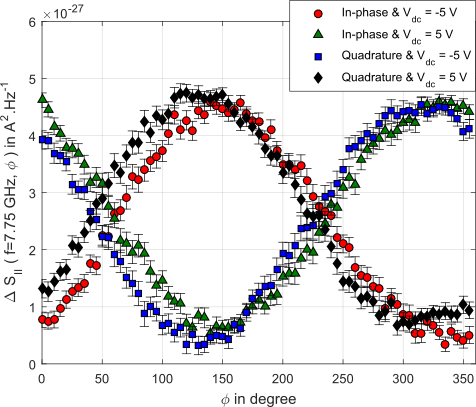
\includegraphics[width = 6.5 cm]{./chap3/RF_noise_vs_pump_phase}
		\end{tabular}
	\end{center}
	
	\caption{\textbf{High frequency noise as a function of pump phase.} The High frequency noise is recorded as a function of the phase difference between the pump and the local oscillator. The two components of the noise are plotted, in red circles and green triangles for in phase components, and in blue squares and black diamonds for quadrature components. For each components two opposite values of bias are applied, a negative bias for red circles and blue squares, and a positive bias for green triangles and black diamonds. The four data set follow a sine curve and the phase of the sine is shifted by $180^{\circ}$ between two different quadratures or two opposite bias.}
	\label{fig: noise pump vs phase}
\end{figure}

In the previous subsection, the high frequency noise generated only by a RF sinus does not depend on the phase difference between the RF sinus and the local oscillator as for the noise generated only by a DC voltage measured in chapter ... .
In the panel (b) of figure Fig.\ref{fig: noise pump vs Vdc}, the noise is generated by both a RF sinus and a DC voltage in this experiment only the difference of noise magnitude are measured but the excess noise is not the simple addition of the contribution of each source.
In this subsection we study the phase dependence of this noise when both RF and DC sources are used, this effect is used in subsection ... to generate and measure a squeezed state.
The set-up used to measure the data points plotted in figure Fig.\ref{fig: noise pump vs phase}, modulate the DC voltage and acquire the real and imaginary parts of the excess noise.
To enhance the effect of the phase dependence, the DC voltage is set at $\pm5$ V at the room temperature source output, which corresponds to approximatively $\pm100$ $\upmu$V applied on the ohmic contact.
The data points are measured every $5^\circ$ of phase values in order to check that the points are placed on a sine function, and two other parameters, the sign of the DC voltage and the real or imaginary component of the excess noise, are changed to check that they are equivalent to a $180^\circ$ phase shift.
The results shown in figure Fig.\ref{fig: noise pump vs phase} follow these trends but with a small asymmetry between the measurements of the real part by the in-phase port and the imaginary part by the quadrature port.  
This measurement allows to calibrate the phase of the local oscillator such that the in-phase noise measurement is minimal for the proper DC voltage.

\subsection{High frequency noise reduction below the noise of a vacuum state}

\begin{figure}[hptb]
	\begin{center}
		\begin{tabular}{c c c c}
			(a) & & (b) & \\
			& 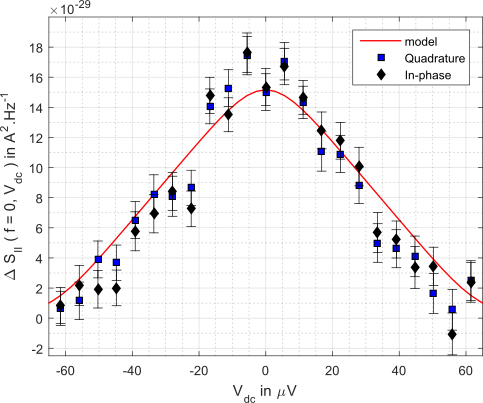
\includegraphics[width = 6.5 cm]{./chap3/LF_noise_squeezed_181206} &
			& 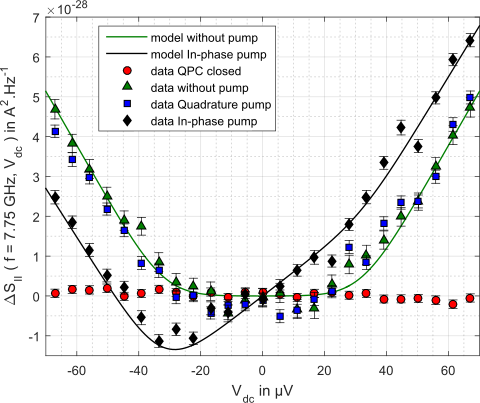
\includegraphics[width = 6.5 cm]{./chap3/RF_noise_squeezed_181206}
		\end{tabular}
	\end{center}
	
	\caption{\textbf{Shot noise as a function of bias voltage with a pump.} \textbf{(a)} Low frequency excess shot noise of the pump is plotted when the pump is in-phase, in black diamond, and in quadrature, in blue square, with the high frequency noise measurement phase reference. The low frequency noise does not depend on the pump phase and they follow the calculated model deduce from the pump Wigner distribution. \textbf{(b)} The high frequency noise is plotted for different parameters of the pump. In red circles the quantum point contact is closed so there is no high frequency noise generated. In green triangles the pump is switched off $V_{\mathrm{ac}} = 0$ V. In blue squares the pump is in quadrature with the noise measurement, the noise measurements are close to the results without pump. In black diamond the pump is in phase with the noise measurement and we measure negative high frequency noise for bias voltage between -20 $\upmu$V and -40 $\upmu$V. Two models are plotted for the high frequency noise without the pump in green line and with the pump in phase in black line.}
	\label{fig: squeezing 181206}
\end{figure}

When the phase of the local oscillator is set thanks to the measurement in the precedent subsection, the DC voltage is swept in a $\pm 60$ $\upmu$V range where the noise reduction is expected.
This subsection explains, with the figure Fig.\ref{fig: squeezing 181206}, the measurement that shows a squeezed state.
The panel (a) of figure Fig.\ref{fig: squeezing 181206}, is a low frequency spectroscopy noise measurement done at the same time as high frequency measurement, and confirms that the amplitude of RF sinus is at $V_{\mathrm{ac}} = 32$ $\upmu$V.
The noise of the RF sinus alone has been precisely measured slightly above this amplitude at $V_{\mathrm{ac}} = 34$ $\upmu$V in previous subsection at $\Delta S_{II} = ...$, so it can be used as a reference and the excess noise is measured compared to this value thanks to the set-up at the bottom part of figure Fig.\ref{fig: set-up chap 3}.
In the panel (b) of figure Fig.\ref{fig: squeezing 181206}, this excess noise is measured for different parameters choices.
The red circles correspond to a choice of central QPC closed, in that situation there is no noise generation even the reference noise is equal to zero.
The green triangles reproduce the measurements of chapter ... in the integer quantum hall regime without RF sinus.
As the experimental set-up measure simultaneously both in-phase and quadrature of the high frequency noise, both measurements are plotted on the graph with blue squares and black diamonds.
The blue squares are the excess noise components which is only the noise of the DC voltage added to the reference noise of the RF pump.
The black diamonds are the measurements which shows the maximal noise variations compared to the DC voltage added noise, and they agree with the model plotted with the black line.
The points for DC voltages between -20 $\upmu$V and -40 $\upmu$V are negatives as expected with the model which means that the noise is smaller than the noise of the RF sinus.
The smallest excess noise value measured is $\Delta S_{II} = ...$, so it is smaller than the noise added to the vacuum by the RF sinus $\Delta S_{II} = ...$, so for smallest excess noise measured the corresponding state is a squeezed state with a component generating less noise than the vacuum state. 

\subsection{Complementary high frequency noise reduction measurements}

\begin{figure}[hptb]
	\begin{center}
		\begin{tabular}{c c c c}
			(a) & & (b) & \\
			& 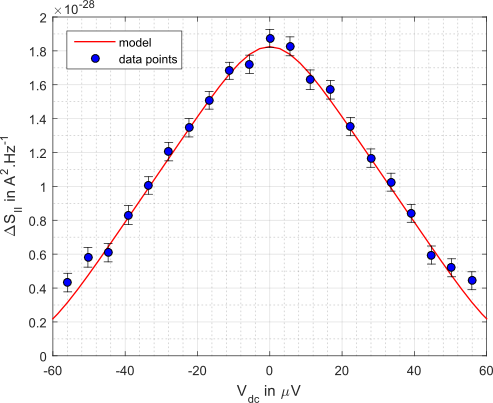
\includegraphics[width = 6.5 cm]{./chap3/LF_noise_squeezed_181112} &
			& 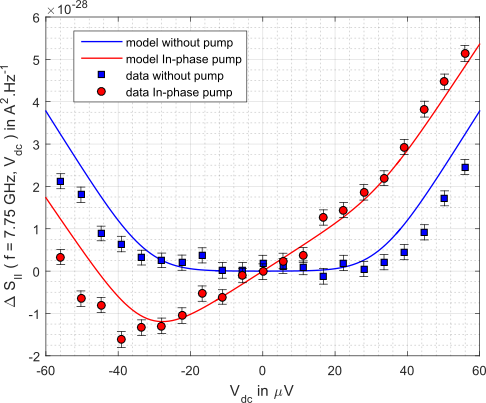
\includegraphics[width = 6.5 cm]{./chap3/RF_noise_squeezed_181112} \\
			(c) & & (d) & \\
			& \includegraphics[width = 6.5 cm]{./chap3/LF_noise_squeezed_181108_300mV} &
			& 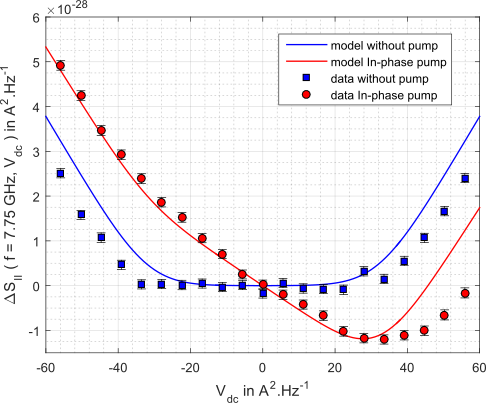
\includegraphics[width = 6.5 cm]{./chap3/RF_noise_squeezed_181108_300mV} \\
			(e) & & (f) & \\
			& \includegraphics[width = 6.5 cm]{./chap3/LF_noise_squeezed_181108_450mV} &
			& \includegraphics[width = 6.5 cm]{./chap3/RF_noise_squeezed_181108_450mV}
		\end{tabular}
	\end{center}
	
	\caption{\textbf{High frequency noise as a function of bias voltage.} In this graph other measurements of low and high frequency noise are performed with pump voltage of higher amplitude. In panels (a) (c) and (e) the excess low frequency noise of the pump is plotted. In panels (b) (d) (f) the high frequency noise is plotted, in blue square the noise is generated by the DC bias only $V_{\mathrm{ac}} = 0$, in red circles the noise is generated by the DC bias and the pump in phase with phase reference voltages. For each panel on the same line the low frequency noise and high frequency noise are measured simultaneaously, so (a) is paired with (b), (c) with (d), and (e) with (f). The models in red lines are deduce from the Wigner distribution of the pumps and numerical calculations. }
	\label{fig: additional squeezing}
\end{figure}

The measurement of negative high frequency excess noise is repeated for higher amplitude of the RF sinus.
These measurements are summarized in figure Fig.\ref{fig: additional squeezing}, each line of the graph corresponds to one measurement with on the left panel the low frequency noise and on the right panel the high frequency noise. 
Panels (a) and (c) show that panels (b) and (d) have the same RF sinus amplitude $V_{\mathrm{ac}} = 36$ $\upmu$V, the RF sinus have just a phase difference of $\pi$ which explains that negative excess noise appear for positive DC voltage on panel (d).
The noise of a RF sinus alone is measured for a closed amplitude of $V_{\mathrm{ac}} = 38$ $\upmu$V at $\Delta S_{II} = ...$.
On panels (b) and (d) some negative points are placed at $\Delta S_{II} = ...$, so a squeezed state is present at these parameters but some data points do not agree with the model at the edge of the DC voltage range.
The two last panels (e) and (f) show an higher amplitude RF sinus with a low frequency noise of $3.5\times 10^{28}$ A$^2$.Hz$^{-1}$ at zero DC voltage, so its amplitude is around $V_{\mathrm{ac}} = 52$ $\upmu$V thanks to figure Fig.\ref{fig: noise pump vs amp} panel (a).
At this high amplitude the noise of the RF sinus alone has been approximatively measured at $\Delta S_{II} = ...$.
On panel (f) the excess noise is negative and reaches a lowest value of $\Delta S_{II} = ...$, this value is lower than previous high frequency noise but the noise of the RF pump is higher.

\begin{equation}
S_{II}\left(\epsilon\right) = \int_{fc-\Delta f/2}^{fc+\Delta f/2}S_{II}\left(\epsilon,f\right)df
\end{equation}

\begin{equation}
S_{II}\left(\epsilon,f\right) = S_{0}\left(\epsilon,f\right)+S_{pump}\left(\epsilon,f\right)
\end{equation}

\begin{equation}
S_{0}\left(eV,f\right) = 2\frac{e^{2}}{h}k_{B}T\left(\frac{eV-hf}{2k_{B}T}\coth\left(\frac{eV-hf}{2k_{B}T}\right)+\frac{eV+hf}{2k_{B}T}\coth\left(\frac{eV+hf}{2k_{B}T}\right)-\frac{hf}{k_{B}T}\coth\left(\frac{hf}{2k_{B}T}\right)\right)
\end{equation}

\begin{equation}
S_{pump}\left(eV,f\right) = \frac{1}{T}\int_{0}^{T} \left(N\left(eV,hf,t\right)+N\left(eV,-hf,t\right)+2\cos\left(4\pi ft+2\phi\right)N\left(eV,0,t\right)\right)dt
\end{equation}

\begin{equation}
N\left(eV,hf,t\right) = \frac{e^{2}}{h}\int_{-\infty}^{+\infty}g\left(eV,hf,\epsilon\right)\Delta W_{pump}\left(\epsilon,t\right)d\epsilon
\end{equation}

\begin{equation}
g\left(eV,hf,\epsilon\right) = 1-f\left(\epsilon-hf+eV\right)-f\left(\epsilon+hf+eV\right)
\end{equation}

\begin{equation}
\Delta S_{II}\left(f = 0, V_{\mathrm{ac}}\right) = \frac{2e^{2}}{h}\sum_{n = -\infty}^{n = +\infty} J_{n}\left(\frac{eV_{\mathrm{ac}}}{hf}\right)^{2}nhf\coth\left(\frac{nhf}{2k_{\mathrm{B}}T_{\mathrm{elec}}}\right)-4\frac{e^{2}}{h}k_{\mathrm{B}}T_{\mathrm{elec}} \label{eq: LF noise vs pump amp}
\end{equation}

where $J_{n}$ are Bessel functions.


%\begin{figure}[hptb]
%	\begin{center}
%		\begin{tabular}{c c c c}
%			(a) & & (b) & \\
%			& \includegraphics[width = 6.5 cm]{./chap3/LF_noise_squeezed_181108_300mV} &
%			& 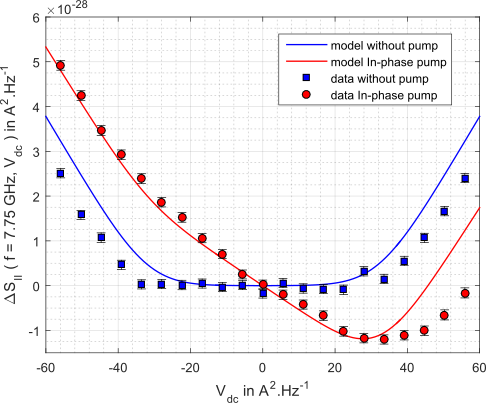
\includegraphics[width = 6.5 cm]{./chap3/RF_noise_squeezed_181108_300mV}
%		\end{tabular}
%	\end{center}
%	
%	\caption{\textbf{High frequency noise as a function of bias voltage.}}
%	\label{fig: squeezing 181108 300mV}
%\end{figure}

%\begin{figure}[hptb]
%	\begin{center}
%		\begin{tabular}{c c c c}
%			(a) & & (b) & \\
%			& \includegraphics[width = 6.5 cm]{./chap3/LF_noise_squeezed_181108_450mV} &
%			& \includegraphics[width = 6.5 cm]{./chap3/RF_noise_squeezed_181108_450mV}
%		\end{tabular}
%	\end{center}
%	
%	\caption{\textbf{High frequency noise as a function of bias voltage.}}
%	\label{fig: squeezing 181108 450mV}
%\end{figure}

%\begin{enumerate}
%	\item simu avec aspect électronique Wigner
%	\item simu avec aspect bosons
%	\item mesure de bruit RF
%	\item interprétation en terme de squeezing
%\end{enumerate}

%\section{\texorpdfstring{Description avec edge-magnetoplasmon}{}}

%\section{\texorpdfstring{Calculs du squeezing avec aspects electron/bosons}{}}

%\section{\texorpdfstring{Comment on le mesure avec bruit RF}{}}

%\section{\texorpdfstring{Résultats en terme de squeezing}{}}

%% !TeX encoding = UTF-8
% !TeX spellcheck = en_GB
% !TeX root = mythesis.tex
\chapter{Conclusion}

Some conclusion text





\appendix
%% !TeX encoding = UTF-8
% !TeX spellcheck = en_GB
% !TeX root = mythesis.tex
\chapter{Complementary charge measurements}

%The  Fith appendix

\section{In strong backscattering}

\section{At filling factor one}

\begin{figure}[hptb]
	\begin{center}
		\begin{tabular}{c c c c}
			(a) & & (b) & \\
			& 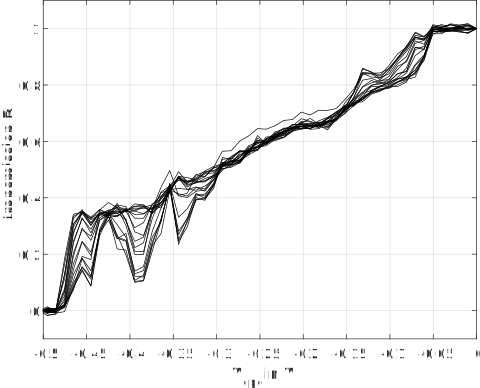
\includegraphics[width = 6.5 cm]{./appE/nu_1_D_vs_Vqpc_for_several_Vdc} &
			& 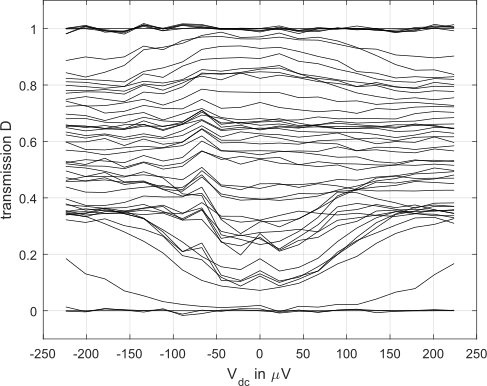
\includegraphics[width = 6.5 cm]{./appE/nu_1_D_vs_Vdc_for_several_Vqpc} \\
			(c) & & (d) & \\
			& 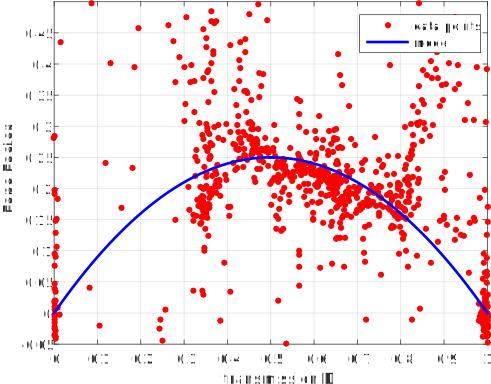
\includegraphics[width = 6.5 cm]{./appE/nu_1_noise_vs_D_for_several_Vdc} &
			& 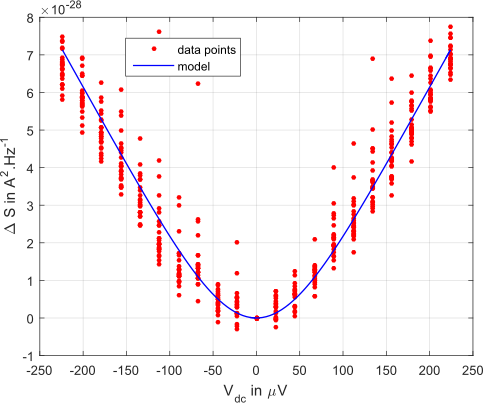
\includegraphics[width = 6.5 cm]{./appE/nu_1_noise_vs_Vdc_for_D_0_4_0_8}
			
		\end{tabular}
	\end{center}
	
	\caption{LF charac at 1}
	\label{fig: LF charac at 1}
\end{figure}

%% !TeX encoding = UTF-8
% !TeX spellcheck = en_GB
% !TeX root = mythesis.tex
\chapter{Bayesian approach for deconvolution in electronic tomography \label{sec: Bayesian approach for deconvolution in electronic tomography}}

%The  first appendix

\section{\texorpdfstring{The deconvolution problem}{The deconvolution problem}\label{sec: The deconvolution problem}}

%présenter le problème

%présenter le domaine

%This problem of inverting an ill-posed problem is also present in other situation such as image deblurring, reconstruction. We benefit from these developpement to adapt and apply it to our specific case.


\subsection{\texorpdfstring{The deconvolution in our specific case}{The deconvolution in our specific case}}

In our measurement protocol, we don't performed a direct measurement of the quantity of interest $\Delta W_{\mathrm{S}}$. Indeed by measuring overlaps between the search quantity $\Delta W_{\mathrm{S}}$ and probes $\Delta W_{\mathrm{P}}$, we only have access to convoluted results. These convolution products are expressed in equations \eqref{eq: convolution spectro} \eqref{eq: convolution real part tomo} \eqref{eq: convolution imag part tomo} and can be modelled by a linear product with a matrix $H$. In addition some measurement noise $N$ is added and the data are obtained following the schematic in figure Fig. \ref{fig: direct model}, where first the searched quantity is convoluted by the matrix $H$, than some noise $N$ is added, and we end up with the measured excess noise $\Delta S$.

\begin{figure}[h]
	\centering
	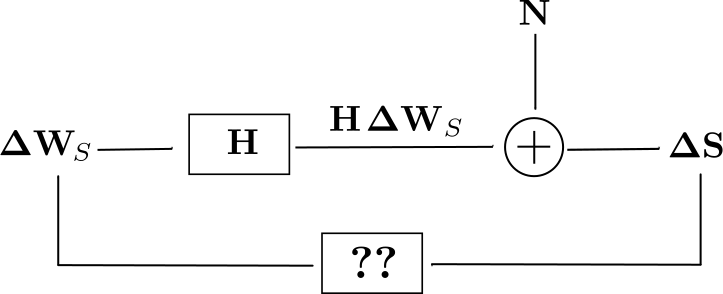
\includegraphics[width = 7cm]{./appA/direct_model}
	\caption{\textbf{Schematic representation of the direct model.} The measured excess noise is modelled as the convolution by a probe function plus some additional noise $N$. In this case we replace the convolution product by its equivalent matrix product $H$. The issue of this annex is to propose what can replace the question marks, and recover $\Delta W_{S}$ from $\Delta S$.}
	\label{fig: direct model}
\end{figure}

This schematic is the direct model and can be summarised in following equation \eqref{eq: direct model} :

\begin{equation}
\Delta S = H\Delta W_{\mathrm{S}}+N \label{eq: direct model}
\end{equation}

The problem is how to find $\Delta W$ for the measurement of $\Delta S$, as depict by the question marks in figure Fig. \ref{fig: direct model}. In other words it is how to inverse the direct model equation \eqref{eq: direct model}.



\subsection{\texorpdfstring{Why do we need a deconvolution method?}{Why we need a deconvolution method?}}

To support the explanation in this annex we can take the example of a 2GHz sine excitation at a temperature of 60mK and carrying one elementary charge e or -e per half-period. And we can focus on the deconvolution of its spectroscopy (or 0$^{\mathrm{th}}$ harmonic) measurement and the results on the whole Wigner function. To estimate the accuracy of different methods, we can compare the data get from measurements with ones get from theoretical calculations shown in figure Fig. \ref{fig: Theory}.

\begin{figure}[hptb]
	\begin{center}
		\begin{tabular}{c c}
			(a) &  \\ 
			
			& 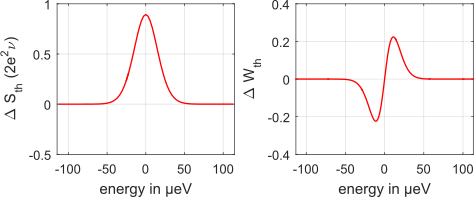
\includegraphics[width = 10 cm]{./appA/Th_result} \\
			
			(b) &  \\ 
			
			& 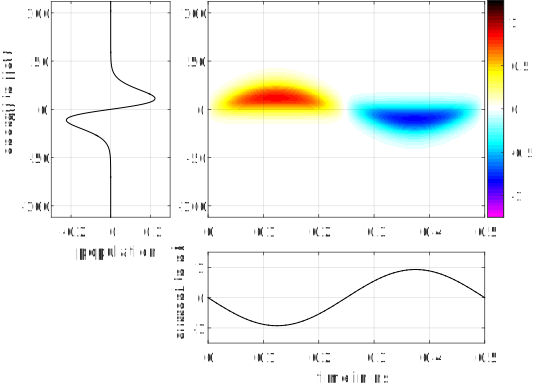
\includegraphics[width = 10 cm]{./appA/Th_wigner}
		\end{tabular} 
	\end{center}
	
	\caption{\textbf{Theoretical calculations on 2GHz sine example at a temperature of 60mK.} \textbf{(a)} left - Calculated theoretical noise $\Delta S_{\mathrm{th}}$ - right - Calculated theoretical spectroscopy $\Delta W_{\mathrm{th}}$. \textbf{(b)} The whole calculated theoretical Wigner function.}
	\label{fig: Theory}
\end{figure}


A naive approach is to discard the unknown noise and to just invert the known convolution matrix $H$, as represented in schematic (a) of figure Fig. \ref{fig: naive deconvolution}. If we look at the estimated result $H^{-1}\Delta S$ in figure Fig. \ref{fig: naive deconvolution} right graph of (b) panel, one can clearly remark that the estimator is dominated by only few oscillations. This result is clearly not reliable since these oscillations are several orders of magnitude stronger than expected result $\Delta W_{\mathrm{th}}$. This effect is not due a limited numerical precision in matrix inversion, because the re-convolution of the estimated solution $H\Delta W$ matches perfectly with the measured data $\Delta S$. The left graph of (b) panel in figure Fig. \ref{fig: naive deconvolution} shows this perfect agreement between $\Delta S$ and $H\Delta W$. Moreover the estimator is sensible to small error perturbations. In figure Fig. \ref{fig: naive deconvolution} panel (c), we add a small noise on measured data to get two very close data set $\Delta S$ and $\Delta S^{\prime}$. These two data set are barely discernible in left graph. But the two respectively estimated results $\Delta W$ and $\Delta W^{\prime}$ are very different. The last remark is that it also does not verify physical properties such as the Pauli exclusion principle for this spectroscopy measurement. The Pauli exclusion principle implies that the result $\Delta W$ plus the Fermi distribution $f_{\mathrm{fermi}}$ should be bounded between 0 and 1 as expressed by equation \eqref{eq: Pauli exclusion principle}:

\begin{equation}
	0 \leq \Delta W_{0}\left(E\right)+f_{\mathrm{fermi}}\left(E\right) \leq 1 \label{eq: Pauli exclusion principle} 
\end{equation}

And values on right graphs of figure Fig. \ref{fig: naive deconvolution} of the order of $10^{4}$ obviously violate the above inequality.

\begin{figure}[hptb]
	\begin{center}
\begin{tabular}{c c}
	(a) &  \\ 
	
	& 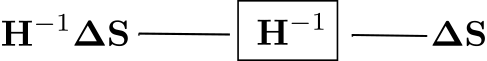
\includegraphics[width = 5cm]{./appA/naive_deconvolution} \\ 
	 
	(b) &  \\ 
	
	& 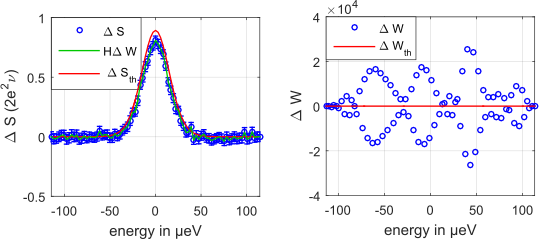
\includegraphics[width = 10 cm]{./appA/Naive_method_results} \\
	(c) &  \\ 
	
	& 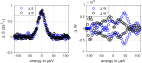
\includegraphics[width = 10 cm]{./appA/Naive_method_results_bis} 
\end{tabular} 
\end{center}
\caption{\textbf{Naive deconvolution method.} \textbf{(a)} Schematic of the naive inverse technique which just consists in multiplying experimental data by the inverse matrix $H^{-1}$. \textbf{(b)} left - Measured data $\Delta S$, calculated theoretical noise $\Delta S_{\mathrm{th}}$ and re-convoluted solution $H\Delta W$, all take similar values - right - Solution of the naive deconvolution $\Delta W$ which is order of magnitude greater than the theoretical solution $\Delta W_{\mathrm{th}}$. \textbf{(c)} left - Two measured data set $\Delta S$ and $\Delta S^{\prime}$ to which are added a random noise. These two data set take similar values. - right - Solution $\Delta W$ based on data points $\Delta S$, and solution $\Delta W^{\prime}$ based on data points $\Delta S^{\prime}$. These two solutions are very different even if the input data points are similar.}
\label{fig: naive deconvolution}
\end{figure}


This behaviour is explained by the fact that deconvolution is an ill-posed problem. This means that the $H$ matrix that model the convolution has some zero or close to zero eigenvalues. This can be shown in the Fourier space where the convolution is just the product by the Fourier transform of the convolution function $h$. And the Fourier transform components of $h$ posses some zeros or close to zero values. So inverting $H$ is equivalent to divide some Fourier component of $\Delta S$ per 0. Even if $H\Delta W$ vanishes for these components, the noise $N$ doesn't and the solution is completely dominated by these noise terms divided by 0.

\section{\texorpdfstring{The Fourier space technique: Wiener filter}{The Fourier space technique: Wiener filter}\label{sec: Wiener filter}}

%présenter technique wiener filtering

\subsection{\texorpdfstring{The optimal Wiener filter in ideal case}{The optimal Wiener filter in ideal case}}

The first technique to overcome the problem presented in above section \ref{sec: The deconvolution problem}, the Wiener filter \cite{wiener1949extrapolation}, is to filter the problematic Fourier components where the noise is divided by 0. The idea is to find the optimum filter that  gives the minimum distance between filtered result $FH^{-1}\Delta S$ and the original signal $\Delta W$. This distance has to be minimum for the average, denoted by $\left<.\right>$ over all different realization of the noise $N$ since it is unknown. This distance is given by \eqref{eq: Wiener criterion}.

\begin{equation}
	\left<\left|\left| FH^{-1}\Delta S - \Delta W \right|\right|_{2}^{2}\right> \label{eq: Wiener criterion}
\end{equation}

In Fourier space the filter $F$ and the matrix $H$ are diagonal, keeping the same symbols for thier diagonal part, we can find the optimum filter $F$ by solving the below equation \eqref{eq: Wiener developpement}.

\begin{equation}
	\frac{\mathrm{d}}{\mathrm{d}F}\left( \left<\left|\left| FH^{-1}\Delta S - \Delta W \right|\right|_{2}^{2}\right> \right) = 0 \label{eq: Wiener developpement}
\end{equation}

which gives the expression of the filter \eqref{eq: optimal Wiener filter}.

\begin{equation}
	F = \frac{HH^{\ast}}{HH^{\ast}+\left<\left|\frac{N}{\Delta W}\right|^{2}\right>} = \frac{1}{1+\left<\left|\frac{N}{H\Delta W}\right|^{2}\right>} \label{eq: optimal Wiener filter}
\end{equation}

This Wiener filter \cite{wiener1949extrapolation} is optimal because:
\begin{itemize}
	\item in the case of a convoluted signal higher than the noise $N\ll H\Delta W$ we get $\Delta S \sim H\Delta$. So we don't need to filter since $H^{-1}\Delta S \sim \Delta W$. This is indeed the case because in this limit $F \sim 1$.
	\item in the other case, the convoluted signal is smaller than the noise $H\Delta W\ll N$. This implies that we measure only noise $\Delta S \sim N$. The filter suppress this term since in this limit $F \sim \left<\left|\frac{H\Delta W}{N}\right|^{2}\right> \ll 1$.
\end{itemize}

\subsection{\texorpdfstring{The implemented Wiener filter}{The implemented Wiener filter}}

To construct this filter we need two quantities, first the noise spectrum $\left<\left|N\right|^{2}\right>$, which is measured if we assumed a white noise and thanks to repeated measurement. The second quantity is the spectrum of the solution $|\Delta W|^{2}$. But as it is the one we are looking for, we don't know it. So we need to use some hypothesis to approach the optimum filter. To do so the first one is that when $\Delta S \gg N$ we can assume $\Delta W \sim H^{-1}\Delta S$ and so the filter has the form \eqref{eq: Wiener filter use for high SNR}:

\begin{equation}
	F = \frac{1}{1+\left<\left|\frac{N}{\Delta S}\right|^{2}\right>} \label{eq: Wiener filter use for high SNR}
\end{equation}

When $\Delta S \sim N$ we know that $H\Delta W \leq N \sim \Delta S$ so we assumed that there is a corner point where $\Delta W \leq \Delta W(\tau_{c}) \sim \frac{\Delta S(\tau_{c})}{H(\tau_{c})}  \sim \frac{N}{H(\tau_{c})}$ and we use it as a boundary for our filter by replacing $H\Delta W$ by $\frac{HN}{H(\tau_{c})}$ like in \eqref{eq: Wiener filter use for low SNR}:

\begin{equation}
	F = \frac{1}{1+\left|\frac{H(\tau_{c})}{H}\right|^{2}} \label{eq: Wiener filter use for low SNR}
\end{equation}

We end up with the following filter \eqref{eq: Wiener filter used}

\begin{eqnarray}
	F &=& \frac{1}{1+\left<\left|\frac{N}{\Delta S}\right|^{2}\right>}\; \mathrm{when}\; H \geq H(\tau_{c}) \\
	&=& \frac{1}{1+\left|\frac{H(\tau_{c})}{H}\right|^{2}}\; \mathrm{when}\; H \leq H(\tau_{c}) \\ \label{eq: Wiener filter used}
\end{eqnarray}

The implementation of this filter in the deconvolution process sketched in the figure Fig. \ref{fig: Wiener_results} panel (a), gives the results of the two lower panels (b) and (c). On right graph of panel (b), the estimated solution $\Delta W$ is comparable with the computed one $\Delta W_{\mathrm{th}}$. On the left graph of panel (b) the re-convoluted estimator $H\Delta W$ still matches the measured data $\Delta S$, even if we filter the deconvolved estimator. It shows that by filtering we do not alter the information given by our measurements. Some points of $\Delta S$ in the middle of the central peak are distant from the computed $\Delta S_{\mathrm{th}}$, and this might explain why at the peaks location some points of $\Delta W$ are also distant from $\Delta W_{\mathrm{th}}$. An effect which is well reproduced by measured points $\Delta S$, is that at high energies, $\left|E\right|\geq 50 \mu$eV, $\Delta S_{\mathrm{th}}$ is flat at zero value. But the estimator $\Delta W$ or the re-convoluted estimator $H\Delta W$ do not capture this effect and display some small unexpected oscillations at these energies. These oscillations induced some unwanted yellow and cyan spots in the total Wigner function of panel (c) and the current shows some deviations from a sine function.

To compute error bars on the estimators $\Delta W$, we assume a white noise whose power is given by repeated measurement $V_{e}=\left<\Delta S^{2}\right>-\left<\Delta S\right>^{2}$. Than error bars are given by $\sigma = \sqrt{f_{\mathrm{sampling}}\int\limits_{0}^{+\infty}\mathrm{d}\tau \left|\frac{F\left(\tau\right)}{H\left(\tau\right)}\right|^{2}V_{e}}$

\begin{figure}[hptb]
		\begin{center}
		\begin{tabular}{c c}
			(a) &  \\ 
			
			& 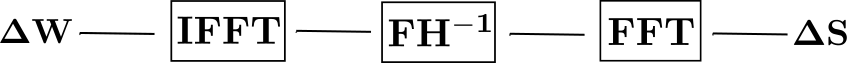
\includegraphics[width = 8 cm]{./appA/Wiener_deconvolution} \\ 
			
			(b) &  \\ 
			
			& 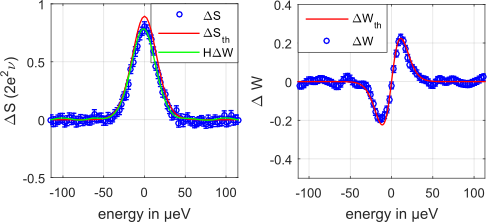
\includegraphics[width = 10 cm]{./appA/Wiener_results} \\
			
			(c) &  \\ 
			
			& 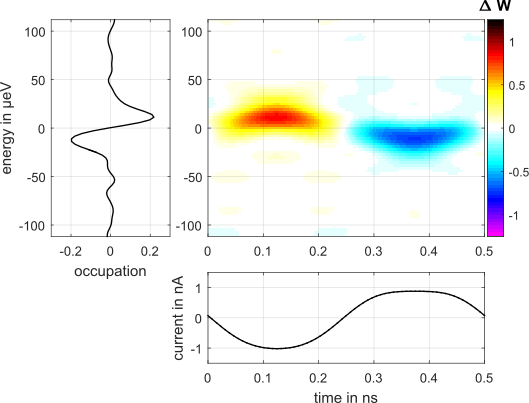
\includegraphics[width = 10 cm]{./appA/Wiener_result_wigner}
		\end{tabular} 
	\end{center}
	\caption{\textbf{Wiener deconvolution filter.} \textbf{(a)} Schematic of Wiener deconvolution technique, the inversion $H^{-1}$ and the filtering $F$ are performed in Fourier space since it is then reduced to a simple product. Indeed in the Fourier basis $H$ is diagonal. \textbf{(b)} left - Measured data $\Delta S$, calculated theoretical noise $\Delta S_{\mathrm{th}}$ and re-convoluted solution $H\Delta W$, all take similar values - right - Solution of the Wiener deconvolution $\Delta W$ which is consistent with expected calculations $\Delta W_{\mathrm{th}}$, except for some oscillations at high energies. \textbf{(c)} The whole Wigner function deduced from measurements thanks to Wiener deconvolution.}
	\label{fig: Wiener_results}
\end{figure}

\section{\texorpdfstring{The Bayesian framework}{The Bayesian framework}}

The Wiener filter in the above section \ref{sec: Wiener filter} gives a reasonable solution compared to the issue raise in figure Fig. \ref{fig: naive deconvolution}. And it has been successfully used for studying electron tomography in \cite{marguerite2017extracting} and \cite{marguerite2017two}. But it can still be improved like for example on the high energy oscillations.

The Wiener technique limitation is as we don't know the power spectrum of the solution, we are forced to use hypothesis that don't correspond to physical properties. To get a solution which verify known physical properties, we introduce a new problem formulation, the Bayesian framework \cite{ayasso2010joint}, \cite{mohammad2015bayesian}, \cite{zhao2016joint}.  The measurement is the mean, or equivalently the maximum, of the probability distribution of $\Delta S$ knowing the searched quantity $\Delta W$ and the variance $V_{e}$ of Gaussian noise $N$. This probability distribution \eqref{eq: likelyhood} is called the likelihood. 

\begin{equation}
	p\left(\Delta S | \Delta W, V_{e} \right) \propto \exp\left(-\frac{1}{2}||\Delta S - H\Delta W||_{V_{e}}^{2}\right)\;\mathrm{with}\;||x||_{V_{e}}^{2} = \sum_{i}^{}\frac{|x_{i}|^{2}}{V_{e,i}} \label{eq: likelyhood}
\end{equation}

But what we are looking for is $\Delta W$. So we are interested in the probability distribution of $\Delta W$ knowing the measurement $\Delta S$ and the noise variance $V_{e}$. Thanks to Bayes'formula \eqref{eq: Bayes'formula} we can link these two probability distributions.

\begin{equation}
	p\left(\Delta W |\Delta S , V_{e} \right)p\left(\Delta S\right) = p\left(\Delta S | \Delta W, V_{e} \right)p\left(\Delta W \right) \label{eq: Bayes'formula}
\end{equation}

We can expressed the probability distribution of interest $p\left(\Delta W |\Delta S , V_{e} \right)$, thanks to the measurement with likelihood $p\left(\Delta S | \Delta W, V_{e} \right)$ and to a prior knowledge on the solution with $p\left(\Delta W \right)$. The a priori informations encoded in the so-called prior distribution function $p\left(\Delta W \right)$ is a much more convenient way to enforce physical properties. For example we choose a Gaussian prior
distribution \eqref{eq: prior distribution annexe} on $\Delta W$

\begin{equation}
p\left( \Delta W \right)  \propto  
\exp\left(
-\frac{1}{2}\left\| \Delta W \right\|^{2}_{V_{f}}  
\right).
\label{eq: prior distribution annexe}
\end{equation}
For variances $V_{f}$, we use the expression \eqref{eq:variances Vf} where $v_f$ and $w$ are parameters tuned to enforce limit condition when energy $\left|E \right|$ increases. This limit condition corresponds to the physical properties that there is less signal at high energy than at low energy.

\begin{equation}
V_{f}\left(E\right) = v_{f}\exp \left( -\frac{E^{2}}{w^{2}} \right)
\label{eq:variances Vf}
\end{equation}

\subsection{\texorpdfstring{Posterior law maximization}{Posterior law maximization}\label{sec: MAP}}

%présenter le framework Bayesian avec MAP

%un peu dire que ce qu'on cherche c'est le max de la loi de probabilité. qu'on peut dire comme a priori qu'on cherche le signal de norme 2 minimum et qu'on préviligie les petites énergies aux grandes. et donc on a juste besoin de trouver le minimum de -log(p) soit du critère J. et que ça on peut le donner analytiquement par ...

In this framework we can define our solution as the most likely $\Delta W$ knowing our measurement points $\Delta S$, their variances $V_{e}$, and the a priori information $V_{f}$. This is the argument which maximise the posterior probability distribution $p\left(\Delta W |\Delta S , V_{e} \right)$. It is equivalent to look for the minimum of the criteria \eqref{eq: MAP criterion}.

\begin{equation}
J\left(\Delta W\right) = - \ln\left(p\left(\Delta W |\Delta S , V_{e} \right)\right) = \frac{1}{2}||\Delta S - H\Delta W||_{V_{e}}^{2}+\frac{1}{2}||\Delta W||_{V_{f}}^{2} \label{eq: MAP criterion}
\end{equation}

Its minimum found by solving $\frac{\mathrm{d}J\left(\Delta W\right)}{\mathrm{d}\Delta W}  = 0$ is the analytical expression \eqref{eq: MAP equation} called maximum a posteriori \cite{fessler1996mean}, \cite{pereyra2017maximum}.

\begin{equation}
\Delta W = F\Delta S = \left(H^{\top}V^{-1}_{e}H+V^{-1}_{f}\right)^{-1}H^{\top}V^{-1}_{e}\Delta S \label{eq: MAP equation}
\end{equation}

On figure Fig. \ref{fig: MAP deconvolution} are plotted the results given by the maximum a posteriori. On the result plotted in the right graph of panel (b) we can noticed that the oscillations at energies $\left|E\right| \geq 50 \mu$eV are suppressed. And also on the Wigner function of panel (c) spots in the same energy range are removed. This effect induced by added a priori information, does not alter the solution found for low energies $\left|E\right| \leq 50 \mu$eV. In addition it also improve in the low energy range the expected electron-hole symmetry. We can remark on panel (b) that the re-convoluted solution $H\Delta W$ looks more symmetric between positive and negative energies. And that the current deduced from the Wigner function in panel (c) is closer to a sine function.

\begin{figure}[hptb]
	\begin{center}
		\begin{tabular}{c c}
			(a) &  \\ 
			
			& \includegraphics[width = 4 cm]{./appA/MAP_deconvolution} \\ 
			
			(b) &  \\ 
			
			& 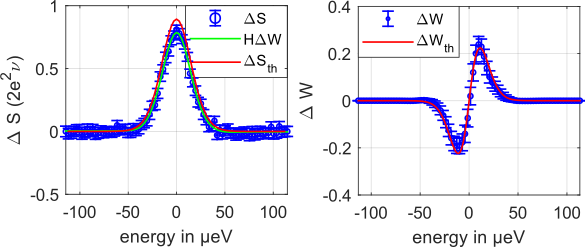
\includegraphics[width = 10 cm]{./appA/MAP_results} \\
			
			(c) &  \\ 
			
			& 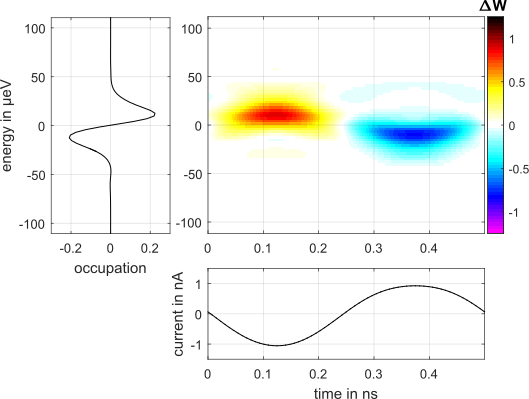
\includegraphics[width = 10 cm]{./appA/MAP_wigner}
		\end{tabular} 
	\end{center}
	
	\caption{\textbf{Maximum A Posteriori deconvolution.} \textbf{(a)} Schematic of MAP deconvolution, the inversion is performed by one matrix product $F$ in the direct space. Some a priori information $V_{f}$ is added to compute the matrix $F$. \textbf{(b)} left - Measured data $\Delta S$, calculated theoretical noise $\Delta S_{\mathrm{th}}$ and re-convoluted solution $H\Delta W$. - right - Solution of the MAP deconvolution $\Delta W$, as expected from $\Delta W_{th}$ the high energy oscillations are suppressed. \textbf{(c)} The whole Wigner function deduced from measurements thanks to MAP. Yellow and blue spots at energies above 50 $\mu$eV are removed.}
	\label{fig: MAP deconvolution}
\end{figure}


We choose as solution the maximum of the posterior distribution to get an analytical formula, but it also corresponds in this case to the mean of the posterior distribution \cite{bardsley2012mcmc} \cite{howard2014sampling}. The panel (a) of figure Fig. \ref{fig: PM_for_MAP} display the solution estimated from the posterior mean, and we can check that it corresponds to the maximum a posteriori. To deduce the posterior mean, we compute the posterior probability distribution, thanks to random draws following the product of likelihood and prior distribution. In panel (b) we plotted for energy point $E$ the histogram of $\Delta W\left(E\right)$ values found. These histograms give a representation of the solution of posterior distribution. We can remark on these histograms that a priori information allows the posterior distribution to be more spread for low energy values $|E|\leq 50 \mu$eV than for higher ones.

\begin{figure}[hptb]
	\begin{center}
		\begin{tabular}{c c}
			(a) &  \\ 
			
			& 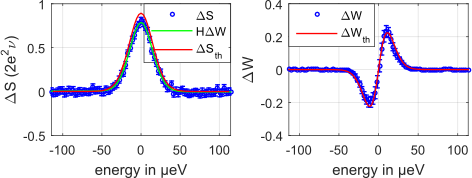
\includegraphics[width = 10 cm]{./appA/PM_for_MAP_posterior_distribution} \\ 
			
			(b) &  \\ 
			
			& 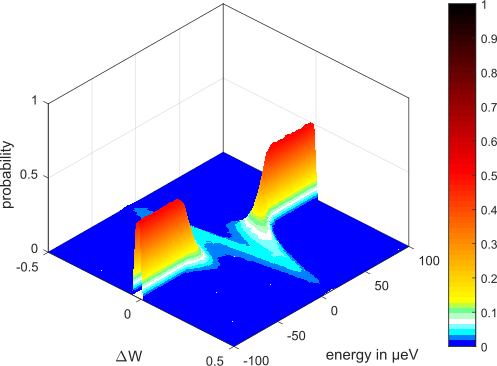
\includegraphics[width = 10 cm]{./appA/MAP_posterior_distribution}
		\end{tabular} 
	\end{center}
	
	\caption{\textbf{Random draws following the posterior distribution.} \textbf{(a)} Solution deduce from the mean of random draws on the posterior distribution. We found the same result as for the maximum a posteriori. \textbf{(b)} Each line along the x-axis is an histogram of solution $\Delta W\left(E\right)$ values for one energy $E$. Values on the z-axis are computed from the percentage of value $\Delta W\left(E\right)$ among the random draws.}
	\label{fig: PM_for_MAP}
\end{figure}


But it does not directly give the error bars plotted on solution $\Delta W$. The error bars correspond to the standard deviation of the deduce $\Delta W$ estimated over different input data $\Delta S$ set with different realization of measurement noise $N$. Whereas the posterior distribution spread is due both to the noise $N$ in the likelihood but also to the prior distribution. Rather than posterior distribution width, the error bars correspond to the fluctuation of its maximum when we add a noise $N$ to the input data set $\Delta S$. To compute these error bars, we performed an analytical calculation of  the covariance matrix $\Sigma_{\Delta W}$ of $\Delta W$ \eqref{eq: MAP covariance} thanks to the analytical expression \eqref{eq: MAP equation}, \cite{fessler1996mean}.

\begin{equation}
\Sigma_{\Delta W} = \left<\Delta W^{2}\right>-\left<\Delta W\right>^{2} = \left(H^{\top}V^{-1}_{e}H+V^{-1}_{f}\right)^{-1}H^{\top}V^{-1}_{e}H\left(H^{\top}V^{-1}_{e}H+V^{-1}_{f}\right)^{-1} \label{eq: MAP covariance}
\end{equation}

This covariance matrix $\Sigma_{\Delta W}$ is plotted on the right of figure Fig. \ref{fig: MAP_covariance}. It is consistent with the covariance matrix plotted on its left, which is computed thanks to random draws of measurement points $\Delta S$ plus a realization of noise $N$. We use only the analytic covariance matrix diagonal part to plot error bars on graphs. But to compute the error bars of extracted quantity from the whole Wigner function such as populations, we use the full covariance matrix.

\begin{figure}[hptb]
	\begin{center}		
	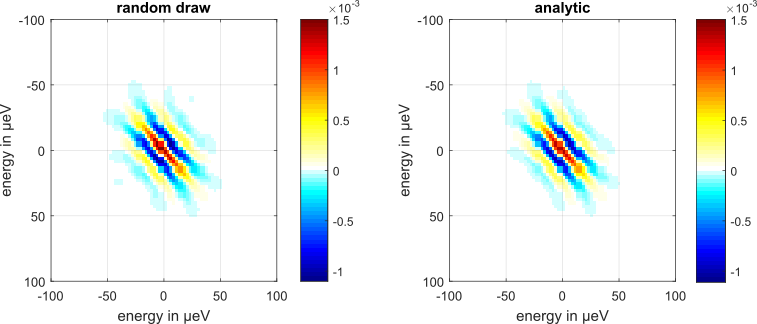
\includegraphics[width = 12 cm]{./appA/MAP_covariance}
	\end{center}
	\caption{\textbf{Covariance matrix of Maximum a posteriori solution.} left - covariance matrix estimated for random draws of input data $\Delta S$ plus a drawn noise $N$ - right - covariance matrix estimated by analytical calculation. These two methods show the same results.}
	\label{fig: MAP_covariance}
\end{figure}


%aidez la présentation avec le direct sampling

%dire qu'on peut faire un tirage au sort pour avoir l'histogramme de valeurs qui suit la loi de la distribution a posteriori et montrer que ça donne le même résultat

%dire qu'on peut aussi donner des barres d'erreur en calculant tout simplement ... mais que attention c'est pas la même chose que la largeur de loi a posteriori, c'est la variation du maximum de la loi a posteriori.

\subsection{\texorpdfstring{Unsupervised technique with joint posterior law maximization}{Unsupervised technique with joint posterior law  maximization}\label{sec: JMAP}}

%présenter le un-supervised avec JMAP

In the above method we impose the values of $V_{f}$, but we don't know their values, so we can replace it by an inverse-gamma probability distribution  law \eqref{eq: hyper-priors inverse gamma law} of shape parameter $\alpha$ and scale $\beta$.

\begin{equation}
p\left(V_{f}|\alpha, \beta \right) \propto \left(\frac{1}{V_{f}}\right)^{\alpha+1}\times\exp\left(-\frac{-\beta}{V_{f}}\right) \label{eq: hyper-priors inverse gamma law}
\end{equation}

What we are now searching is the most likely values of $\Delta W$ and $V_{f}$ knowing measurements points $\Delta S$, their variances $V_{e}$, and parameters $\alpha$, $\beta$. So the posterior law \eqref{eq: JMAP posterior law} is re-expressed due to Bayes'rule.

\begin{equation}
p\left(\Delta W, V_{f} |\Delta S , V_{e}, \alpha, \beta \right) \propto p\left(\Delta S | \Delta W, V_{e} \right)p\left(\Delta W | V_{f} \right)p\left(V_{f} | \alpha, \beta\right) \label{eq: JMAP posterior law}
\end{equation}

To converge towards both $\Delta W$ and $V_{f}$ which maximise the posterior, we performed an alternate optimization of $p\left(\Delta W |\Delta S , V_{e}, V_{f} \right)$ and $p\left(V_{f} |\Delta S , V_{e},\Delta W  \right)$ \cite{mohammad2015bayesian}, \cite{ayasso2010joint}, \cite{zhao2016joint}. This joint maximization is performed by alternatively updating the value of $\Delta W$ as previously thanks to formula \eqref{eq: MAP equation}, than updating the value of $V_{f}$ thanks to formula \eqref{eq: Vf updates formula}.

\begin{equation}
V_{f} = \frac{\beta+\frac{1}{2}\Delta W^{2}}{\alpha+\frac{3}{2}} \label{eq: Vf updates formula}
\end{equation}

For this new method, formula \eqref{eq: prior distribution} is only used to initialize $V_{f}$ and $\beta = \left(\alpha+1\right)V_{f}$. The value of $\alpha$ determines the closeness of the optimized $V_{f}$ to initialization \eqref{eq: prior distribution}.

On figure Fig. \ref{fig: JMAP deconvolution}, we remark that in this JMAP case there are almost no difference with above MAP technique section \ref{sec: MAP}.

\begin{figure}[hptb]
	\begin{center}
		\begin{tabular}{c c}
			(a) &  \\ 
			
			& \includegraphics[width = 4 cm]{./appA/JMAP_deconvolution} \\ 
			
			(b) &  \\ 
			
			& 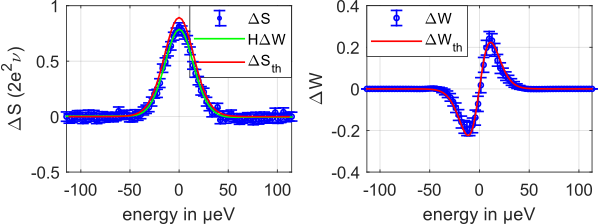
\includegraphics[width = 10 cm]{./appA/JMAP_result} \\
			
			(c) &  \\ 
			
			& 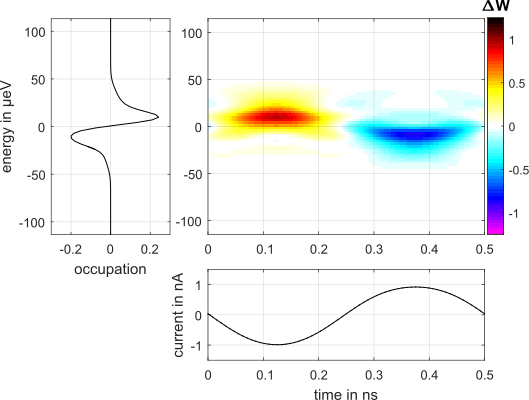
\includegraphics[width = 10 cm]{./appA/JMAP_wigner}
		\end{tabular} 
	\end{center}
	
	\caption{\textbf{Joint Maximum A Posteriori deconvolution.} \textbf{(a)} Schematic of JMAP deconvolution, the inversion is performed by one matrix product $F$ in the direct space. The solution is used to optimize the values of $V_{f}$ parameters, which follow an Inverse-Gamma law of shape parameter $\alpha$ and scale parameter $\beta$. After several loop step between $F$ and $V_{f}$ we get the solution $F\Delta S$. \textbf{(b)} left - Measured data $\Delta S$, calculated theoretical noise $\Delta S_{\mathrm{th}}$ and re-convoluted solution $H\Delta W$. - right - Solution of the JMAP deconvolution $\Delta W$, which is similar to the solution given by the MAP method. \textbf{(c)} The whole Wigner function deduced from measurements thanks to JMAP.}
	\label{fig: JMAP deconvolution}
\end{figure}


%The schematics of this algorithm is show on figure \ref{fig: JMAP deconvolution}. This gives the results show in figure \ref{fig: JMAP deconvolution}.

%aidez la présentation avec la Monte-Carlo-Markov-Chain ou pas

\subsection{\texorpdfstring{Box constrained problem with projected gradiant}{Box-constraint problem with projected gradiant}}

%présenter la box-constraint et le gradient projeté

The above technique allows to add some a priori information like a high energy cut-off. But still some physical properties are missing. The ones added in this section is the Pauli exclusion principle and the Cauchy-Schwartz inequality \cite{ferraro2013wigner}. The Pauli exclusion principle enforces that the result of the 0$^{\mathrm{th}}$ harmonic of the Wigner function (or spectroscopy) plus the Fermi distribution has to be bounded between 0 and 1, see equation \eqref{eq: Pauli exclusion principle}. This inequality condition define a box in which the solution has to be found. This kind of problem is common in image processing, where grey pixel values are bounded between 0 and 255, it is called a box-constrained problem \cite{afonso2011augmented} \cite{lanteri2002penalized} \cite{chan2012multiplicative} \cite{bardsley2012mcmc2}. To look for a solution inside the box defined by the Pauli exclusion principle, we perform a projected gradient descent method \cite{figueiredo2007gradient} \cite{bertsekas1997nonlinear}.

This method follows the drawing of figure Fig. \ref{fig: ProjGrad descent}. First we initialize the solution by projecting the maximum a posteriori solution $\Delta W_{\mathrm{MAP}}$ given by equation \eqref{eq: MAP equation} inside the box by \eqref{eq: solution projection inside box}.

\begin{eqnarray}
\Delta W_{\mathrm{init}} = \min\left(\max\left(\Delta W_{\mathrm{MAP}} ,-\mathrm{fermi} \right),1-\mathrm{fermi} \right)  \label{eq: solution projection inside box}
\end{eqnarray}

The criterion $J\left(\Delta W\right)$ \eqref{eq: MAP criterion} gives the value we have to minimize. So we can compute its gradient $\nabla J\left(\Delta W\right)$ \eqref{eq: gradient} at the previous value of $\Delta W_{\mathrm{init}}$.

\begin{equation}
\nabla J\left(\Delta W_{\mathrm{init}}\right) = -H^{\top}V^{-1}_{e}\left(\Delta S-H\Delta W_{\mathrm{init}}\right)+V^{-1}_{f}\Delta W_{\mathrm{init}} \label{eq: gradient}
\end{equation}

And project it to stay in the box by setting at zero all components that point outside of the box when $\Delta W_{\mathrm{init}}$ is at a boundary of the box. We can also compute the optimum displacement along direction given by the gradient computed in \eqref{eq: gradient}, and performed one descent step to find $\Delta W_{\mathrm{Proj.Grad.}}$. Than as in the previous section \ref{sec: JMAP} we performed an alternate optimization by updating the values of $V_{f}$ thanks to formula \eqref{eq: Vf updates formula}. To perform the whole descent we return to the gradient calculation step to perform several iteration until the joint posterior law is maximized under the box constraints imposed by Pauli exclusion principle. For harmonics one to five, the box boundary are given by the solution of the zero harmonic thanks to Cauchy-Schwartz inequality.

This algorithm gives the result in figure Fig. \ref{fig: ProjGrad deconvolution}. Almost all the un-expected cyan and yellow spots included at low energies have been suppressed, compare to the Wiener filtering result in figure Fig. \ref{fig: Wiener_results}.


\begin{figure}[hptb]
	\centering
	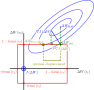
\includegraphics[width = 10 cm]{./appA/gradient_descent_schematics}
	\caption{\textbf{Projected gradient descent schematic.} In red the box given by the Pauli exclusion principle. In blue the criterion given by the posterior distribution law. In green projection for the initial value and the gradient. In gold solution given by the algorithm, which is the lowest value of the criterion in the box given by the Pauli exclusion principle.}
	\label{fig: ProjGrad descent}
\end{figure}

\begin{figure}[hptb]
	\begin{center}
		\begin{tabular}{c c}
			(a) &  \\ 
			
			& \includegraphics[width = 8 cm]{./appA/ProjGrad_deconvolution} \\ 
			
			(b) &  \\ 
			
			& 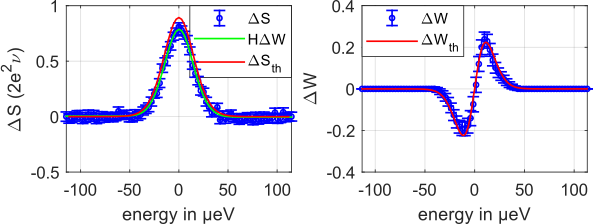
\includegraphics[width = 10 cm]{./appA/PG_result} \\
			
			(c) &  \\ 
			
			& 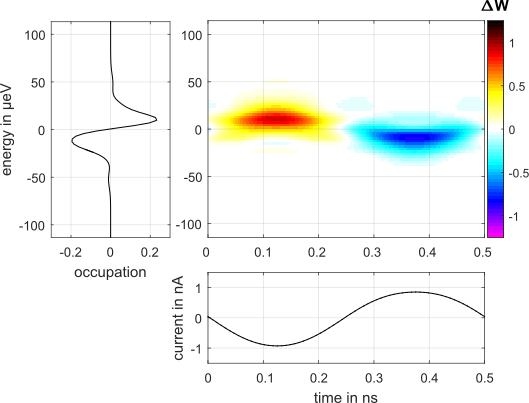
\includegraphics[width = 10 cm]{./appA/PG_wigner}
		\end{tabular} 
	\end{center}
	
	\caption{\textbf{Projected Gradient deconvolution method.} \textbf{(a)} Schematic of the deconvolution method, first a MAP deconvolution is performed. Its solution $F\Delta S$ is projected by $P$ in the box $M$. Than starting from this initial value, one projected gradient descent step and one update of $V_{f}$ values are repeated at each loop step \textbf{(b)} left - Measured data $\Delta S$, calculated theoretical noise $\Delta S_{\mathrm{th}}$ and re-convoluted solution $H\Delta W$. - right - Solution of the deconvolution $\Delta W$. \textbf{(c)} The whole Wigner function deduced from measurements. Almost all unexpected yellow and cyan spots are erased even in the energy range below 50 $\mu$eV.}
	\label{fig: ProjGrad deconvolution}
\end{figure}

\section{\texorpdfstring{Outlook: toward a 2D treatment}{Outlook: toward a 2D treatment}}

%mettre en perspective le full traitement 2D

The Wiener filtering method have already been investigated in the PhD\cite{marguerite2017two}, in this section we develop and demonstrate a more robust method which enable to enforce physical properties on the solution. This improve the deconvolution results especially for signal going to higher energies. But still some improvements can be made. The above method is succession of 1D deconvolution, where we use the first one to impose the Cauchy-Schwartz inequality to all others harmonics as sketch in figure Fig. \ref{fig: 1D->2D deconvolution} panel (a). This is an improvement toward the use of all harmonics, but it is not yet a full 2D deconvolution, where the presence of signal in higher harmonics could suggest that there are some signal at the harmonic 0$^{\mathrm{th}}$. So an improved version could be to deconvolve simultaneously all harmonics as depict in figure Fig. \ref{fig: 1D->2D deconvolution} panel (b).

\begin{figure}[hptb]
	\begin{center}
		\begin{tabular}{c c c c}
			(a) & & (b) &  \\ 
			
			& \includegraphics[scale = 0.25]{./appA/1D_deconvolution} & & 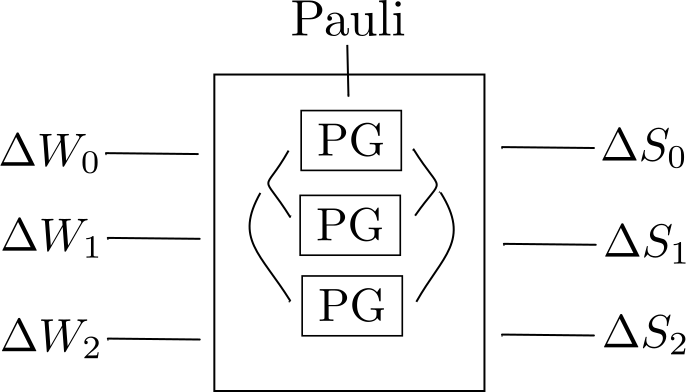
\includegraphics[scale = 0.25]{./appA/2D_deconvolution} 
		\end{tabular} 
	\end{center}

	\caption{\textbf{From 1D to 2D deconvolution.} \textbf{(a)} - succession of 1D Project Gradient deconvolution method used in this manuscript - \textbf{(b)} - perspective of a 2D deconvolution method.}
	\label{fig: 1D->2D deconvolution}

\end{figure}


%% !TeX encoding = UTF-8
% !TeX spellcheck = en_GB
% !TeX root = mythesis.tex
\chapter{Wigner function of different shape pulses}

%The  Third appendix

\section{A sinus shape emitting one electron than one hole}

\subsection{Wigner}

\begin{figure}[hptb]
	\begin{center}
		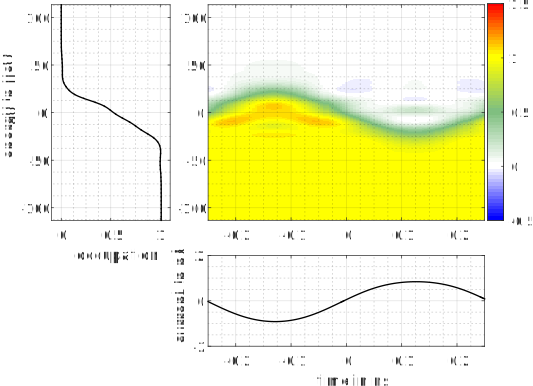
\includegraphics[width = 10 cm]{./appC/wigData_sinus_Projected_Gradient_Method} 
	\end{center}
	
	\caption{Wigner sinus}
	\label{fig: Wigner sinus}
\end{figure}

\subsection{Probabilities and Coherences}

\begin{figure}[hptb]
	\begin{center}
		\begin{tabular}{c c c c}
			(a) & & (b) & \\ 
			& \includegraphics[width = 6.5 cm]{./appC/JnlData_sinus_Projected_Gradient_Method_proba_el} & & 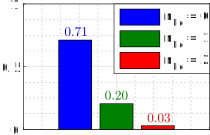
\includegraphics[width = 6.5 cm]{./appC/JnlData_sinus_Projected_Gradient_Method_proba_ho}
		\end{tabular}
	\end{center}
	
	\caption{proba sinus}
	\label{fig: proba sinus}
\end{figure}



\begin{figure}[hptb]
	\begin{center}
		\begin{tabular}{c c c c}
			(a) & & (b) & \\ 
			& \includegraphics[width = 6.5 cm]{./appC/JnlData_sinus_Projected_Gradient_Method_coh_el_el} & & \includegraphics[width = 6.5 cm]{./appC/JnlData_sinus_Projected_Gradient_Method_coh_ho_ho} \\
			(c) & & & \\
			& \includegraphics[width = 6.5 cm]{./appC/JnlData_sinus_Projected_Gradient_Method_coh_el_ho} & & 
		\end{tabular}
	\end{center}
	
	\caption{coherence sinus}
	\label{fig: coherence sinus}
\end{figure}

\subsection{Wavefunctions}

\begin{figure}[hptb]
	\begin{center}
		\begin{tabular}{c c c c}
			(a) & & (b) & \\ 
			& \includegraphics[width = 6.5 cm]{./appC/wannierwigData_sinus_Projected_Gradient_Method-el-0} & & \includegraphics[width = 6.5 cm]{./appC/wannierwigData_sinus_Projected_Gradient_Method-el-1} \\
			(c) & & (d) & \\
			& \includegraphics[width = 6.5 cm]{./appC/wannierwigData_sinus_Projected_Gradient_Method-ho-0} & & \includegraphics[width = 6.5 cm]{./appC/wannierwigData_sinus_Projected_Gradient_Method-ho-1}
		\end{tabular}
	\end{center}
	
	\caption{wannier sinus overlap après rotation de pi/2*0.38 de 0.95 avec des Levitons de largeur 80 ps}
	\label{fig: wannier sinus}
\end{figure}

\section{An asymmetric pulse with exponentially decreasing current \label{sec: An asymetric pulse with exponentially decreasing current}}

\subsection{Wigner}

\begin{figure}[hptb]
	\begin{center}
		\includegraphics[width = 10 cm]{./appC/wigData_exponential_50ps_1e_JMAP_f_vf} 
	\end{center}
	
	\caption{Wigner exponential}
	\label{fig: Wigner exponential}
\end{figure}

\subsection{Probabilities and Coherences}

\begin{figure}[hptb]
	\begin{center}
		\begin{tabular}{c c c c}
			(a) & & &   \\ 
			& \includegraphics[width = 5cm]{./appC/JnlData_exponential_50ps_1e_JMAP_f_vf_proba} &
			&  \\
			(b) & & (c) & \\
			& \includegraphics[width = 5cm]{./appC/JnlData_exponential_50ps_1e_JMAP_f_vf_coh_inter_period} &
			& \includegraphics[width = 5cm]{./appC/JnlData_exponential_50ps_1e_JMAP_f_vf_coh_el_ho}
		\end{tabular} 
	\end{center}
	\caption{(a) pi du exponential (b) coh du exponential}
	\label{fig: Jnl exponantial}
\end{figure}

\subsection{Wavefunctions}

\begin{figure}[hptb]
	\begin{center}
		\begin{tabular}{c c c c}
			(a) & & (b) & \\ 
			& \includegraphics[width = 6.5 cm]{./appC/wannierwigData_exponential_50ps_1e_JMAP_f_vf-el-0} & & \includegraphics[width = 6.5 cm]{./appC/wannierwigData_exponential_50ps_1e_JMAP_f_vf-el-1} \\
			(c) & & & \\
			& \includegraphics[width = 6.5 cm]{./appC/wannierwigData_exponential_50ps_1e_JMAP_f_vf-ho-0} & &
		\end{tabular}
	\end{center}
	
	\caption{wannier exponential}
	\label{fig: wannier exponential}
\end{figure}

\begin{figure}[hptb]
	\begin{center}
		\begin{tabular}{c c c c}
			(a) & & (b) & \\ 
			& \includegraphics[width = 6.5 cm]{./appC/wannierwigData_exponential_50ps_1e_JMAP_f_vf-el-moins-y} & & \includegraphics[width = 6.5 cm]{./appC/wannierwigData_exponential_50ps_1e_JMAP_f_vf-el-plus-y}
		\end{tabular}
	\end{center}
	
	\caption{y axis wannier exponential}
	\label{fig: y axis wannier exponential}
\end{figure}


%% !TeX encoding = UTF-8
% !TeX spellcheck = en_GB
% !TeX root = mythesis.tex
\chapter{Wigner function of different charge per pulse}

%The  Forth appendix

\section{A non integer charge Lorentzian pulse}

\subsection{Wigner}

\begin{figure}[hpbt]
	\centering
	\includegraphics[width = 10cm]{./appD/wigData_leviton_20ps_0_5e_51mK_Projected_Gradient_Method}
	\caption{wigner du 0.5e 25ps}
	\label{fig: wigner du 0.5e 20ps}
\end{figure}

\subsection{Probabilities and Coherences}

\begin{figure}[hptb]
	\begin{center}
		\begin{tabular}{c c c c}
			(a) & & &   \\ 
			& \includegraphics[width = 5cm]{./appD/JnlData_leviton_20ps_0_5e_51mK_Projected_Gradient_Method_proba} &
			&  \\
			(b) & & (c) & \\
			& \includegraphics[width = 5cm]{./appD/JnlData_leviton_20ps_0_5e_51mK_Projected_Gradient_Method_coh_inter_period} &
			& \includegraphics[width = 5cm]{./appD/JnlData_leviton_20ps_0_5e_51mK_Projected_Gradient_Method_coh_el_ho}
		\end{tabular} 
	\end{center}
	\caption{(a) pi du 0.5e 20ps (b) coh du 0.5e 20ps}
	\label{fig: Jnl du 0.5e 20ps}
\end{figure}

\subsection{Wavefunctions}

\begin{figure}[hptb]
	\begin{center}
		\begin{tabular}{c c c c}
			
			(a) & & (b) &  \\ 
			& \includegraphics[width = 6.5 cm]{./appD/wannierwigData_leviton_20ps_0_5e_51mK_Projected_Gradient_Method-el-0} &
			& \includegraphics[width = 6.5 cm]{./appD/wannierwigData_leviton_20ps_0_5e_51mK_Projected_Gradient_Method-el-1} \\
			(c) & & & \\
			& \includegraphics[width = 6.5 cm]{./appD/wannierwigData_leviton_20ps_0_5e_51mK_Projected_Gradient_Method-ho-0} & &
		\end{tabular} 
	\end{center}
	\caption{(a) wannier el-0 du 0.5e 25ps overlap de 0.98 avec leviton \underline{50 ps} (b) wannier el-1 du 0.5e 20ps (c) wannier ho-0 du 0.5e 20ps}
	\label{fig: wannier du 0.5e 20ps}
\end{figure}

\section{An analysis for different charge electron than holes periodic pulses}


%% !TeX encoding = UTF-8
% !TeX spellcheck = en_GB
% !TeX root = mythesis.tex
\chapter{Squeezing using a two harmonic pump}

%The  Fith appendix



%% !TeX encoding = UTF-8
% !TeX spellcheck = en_GB
% !TeX root = mythesis.tex
\chapter{Dilution cryostat wiring}

%The  Second appendix

\begin{figure}[hptb]
	\begin{center}
		\begin{tabular}{c}
			(a) \\ 
			
			\includegraphics[height = 12 cm]{./appB/input_RF_line} 
		\end{tabular}
	\end{center}
	
	\caption{Input RF lines}
	\label{fig: Input RF lines}
\end{figure}

\begin{figure}[hptb]
	\begin{center}
		\begin{tabular}{c}
			(a) \\ 
			
			 \includegraphics[height = 12 cm]{./appB/input_DC_line}
		\end{tabular}
	\end{center}
	
	\caption{Input DC lines}
	\label{fig: Input DC lines}
\end{figure}

\begin{figure}[hptb]
	\begin{center}
		\begin{tabular}{c}
			(a) \\ 
			
			\includegraphics[height = 4 cm]{./appB/power_supply_ampli}
		\end{tabular}
	\end{center}
	
	\caption{amplifier supply lines}
	\label{fig: amplifier supply lines}
\end{figure}


\begin{figure}[hptb]
	\begin{center}
		\begin{tabular}{c}
			(a) \\ 
			
			\includegraphics[height = 12 cm]{./appB/output_LF_line}
		\end{tabular}
	\end{center}
	
	\caption{output LF line}
	\label{fig: output LF line}
\end{figure}

\begin{figure}[hptb]
	\begin{center}
		\begin{tabular}{c}
			(a) \\ 
			
			\includegraphics[height = 18 cm]{./appB/output_RF_noise_line}
		\end{tabular}
	\end{center}
	
	\caption{output RF noise line}
	\label{fig: output RF noise line}
\end{figure}

\begin{figure}[hptb]
	\begin{center}
		\begin{tabular}{c}
			(a) \\ 
			
			\includegraphics[height = 12 cm]{./appB/output_RF_current_line}
		\end{tabular}
	\end{center}
	
	\caption{output RF current line}
	\label{fig: output RF current line}
\end{figure}

\eqref{eq: RF power after one attenuator}
\begin{equation}
P_{f} = DP_{i}+\left(1-D\right)P_{0}\;\&\; P=4k_{B}T\Delta f \label{eq: RF power after one attenuator} 
\end{equation}

\begin{tabular}{|c||c|c|c|}
	\hline 
	Plate name & Plate temperature & attenuator & RF temperature \\ 
	 & (in K) & (in dB) & (in K) \\ 
	\hline
	\hline 
	Room temperature & 300 & 0 & 300 \\ 
	\hline 
	PT1 & 70 & -6 & 128 \\ 
	\hline 
	PT2 & 4 & -10 & 16 \\ 
	\hline 
	Still & 0.8 & -6 & 4.7 \\ 
	\hline 
	Cold & 0.1 & -10 & 0.56 \\ 
	\hline 
	Mixing chamber & 0.02 & -20 & 0.025 \\ 
	\hline 
	Docking station & 0.02 & 0 & 0.025 \\ 
	\hline 
\end{tabular} 
%%%%%%%%%%%%%%%%%%%%%%%%%%%%%% FINAL PAGES %%%%%%%%%%%%%%%%%%%%%%%%%%%%%%%%%%
\backmatter
%%%%%%%%%%%%%%%%%%%%%%%%%%%%  BIBLIOGRAPHY %%%%%%%%%%%%%%%%%%%%%%%%%%%%%%%%%%
\cleardoublepage
\phantomsection
\addcontentsline{toc}{chapter}{Bibliographie}
%%%%% use of BiBTeX:
\bibliographystyle{./bib/thesefr-href}
\bibliography{./bib/shortbib}
%%%%% to be replaced by,  for final version:
%\intput{mythesis.bbl}
%%%%%%%%%%%%%%%%%%%%%%%%%  4th COVER %%%%%%%%%%%%%%%%%%%%%%%%%%%%%%%%%%%%%%%%
%\backcover % requires thcover.sty loaded and thcoverdata.tex filled
\end{document}